\documentclass[a4paper,12pt,twoside]{report}
\usepackage[left=2cm,right=2cm,top=2cm,bottom=3cm]{geometry}

\usepackage{comment}
\usepackage[utf8]{inputenc}
\usepackage{amsmath}
\usepackage[spanish, es-tabla]{babel}
\usepackage{amsfonts}
\usepackage{amssymb}
\usepackage{multirow, array} 
\usepackage{chngcntr}
\usepackage{graphicx}
\usepackage{subfig}
\usepackage{cite}
\usepackage{adjustbox}
\usepackage[table]{xcolor}
\usepackage{float}
\usepackage{listings}
\usepackage[toc,page]{appendix}
\usepackage{color}   %May be necessary if you want to color links
\usepackage{hyperref}
\hypersetup{
    colorlinks=true, %set true if you want colored links
    linktoc=page,     %set to all if you want both sections and subsections linked
    linkcolor=blue,  %choose some color if you want links to stand out
}

\title{}
\begin{document}
\begin{center}
\thispagestyle{empty}
\fontsize{12pt}{12pt}\selectfont 

%%%%%%%%%%%%%%%%%%% PORTADA %%%%%%%%%%%%%%%%%%%%%%%%


\textbf {\huge Diseño e implementación de una estación meteorológica para la medición de campo eléctrico atmosférico en observatorios de rayos cósmicos.}


\vspace{3cm}

{\large \textbf{Autores:}}

\vspace{0.5cm}

\large Pedro Andrés Salgado Meza\\Leonardo Antonio Florez Villegas

\vspace{3cm}
{\large \textbf{Director}}\\
\vspace{0.5cm}
{\large Jesús Peña Rodríguez }\\
\vspace{0.5cm}
{\large \textbf{Codirector}}\\
\vspace{0.5cm}
{\large Luis A. Núñez\\Jaime Barrero Pérez}
\vspace{3cm}


\normalsize
\vspace{2cm}

\large Universidad Industrial de Santander\\

\large  Facultad de Fisicomecánicas \\

\large  Escuela de Ingenierías Eléctrica, Electrónica y de Telecomunicaciones \\
Enero 2020
    
  \end{center}
\large


\newpage
%%%%%%%%%% CONTENIDO %%%%%%%

\tableofcontents % indice de contenidos

%\cleardoublepage
\addcontentsline{toc}{chapter}{Lista de figuras} % para que aparezca en el indice de contenidos
\listoffigures % indice de figuras


%\chapter{Introducción}
Los rayos cósmicos son partículas altamente energéticas que llegan a nuestro planeta tras propagarse por el espacio. Proceden de fenómenos astrofísicos violentos tales como fulguraciones solares o explosiones de supernovas. Cuando un rayo cósmico ingresa a la atmósfera, interactúa con los átomos que la componen creando chubascos de partículas secundarias, también llamados lluvias aéreas extendidas (EAS).\\

Los rayos cósmicos secundarios pueden ser usados en diferentes aplicaciones, que abarcan desde el entendimiento de la naturaleza de los rayos cósmicos primarios, hasta aplicaciones en clima espacial, física de altas energías \cite{Spurio2015}, muongrafía \cite{kaiser2018muography} entre otras.\\

Debido a que la mayoría de partículas generadas en la atmósfera poseen carga, estas pueden ser afectadas por los campos eléctricos presentes durante las tormentas, causando un aumento en el flujo de secundarios a nivel del suelo. Actualmente se han realizado algunos estudios correlacionando ambos fenómenos. Wang et al. \cite{wang2012effect} y Alexeenko et al. \cite{alexeenko2002transient} concluyeron que el número de muones detectados a nivel de suelo es modulado por la magnitud del campo eléctrico atmosférico. Bartoli et al. \cite{bartoli2018observation} observaron un decrecimiento en el número de electrones registrados por ARGO-YBJ durante tormentas eléctricas, mientras que Huang et al. \cite{zhao2019effects} encontraron que la variación en el número de electrones y gammas depende de la polaridad del campo eléctrico atmosférico.\\

Sin embargo, el estudio de eventos transitorios en el flujo de secundarios se ha limitado en profundidad ya que el registro de datos de campo eléctrico atmosférico durante tormentas es escaso en los observatorios de CRs (Rayos Cósmicos). Por esta razón, es necesario conocer la intensidad y las variaciones del campo eléctrico atmosférico con el fin de correlacionar su efecto sobre los transitorios en la tasa de partículas detectadas a nivel de suelo.


%%%%%%%%%%%%%%%%%%% JESUS %%%%%%%%%%%%%%%%%%%%%%%%%%%%%%%%%%%%%%%%%
%La muongrafía es una técnica no-invasiva que se utiliza para estudiar grandes estructuras antrópicas o naturales. Sus aplicaciones van desde detección de materiales ocultos en contenedores \cite{Blanpied2015}, arqueología \cite{Morishima2017, Gmez2016, Alvarez1970}, exploración geológica en Marte \cite{Kedar2013}, inspección de plantas nucleares \cite{Fujii2013}, cavidades subterráneas \cite{Saracino2017} y  vulcanología \cite{Tanaka2005, Tanaka2009, Lesparre2010, Lesparre2011, Lesparre2012}.\\

%Actualmente las herramientas más utilizadas en el estudio de volcanes son la sismología, gravimetría y tomografía eléctrica. Estas tienen una resolución espacial y capacidad de penetración baja \cite{RosasCarbajal2017}, además los datos deben ser registrados de manera directa sobre la superficie del volcán, \cite{Marteau2012}. La muongrafía ofrece una alternativa con resolución espacial de decenas de metros \cite{Lesparre2012}, una gran capacidad de penetración y la adquisición de información es no-invasiva \cite{Nishiyama2014}.\\

%Su funcionamiento se basa en la medición del flujo de muones que cruzan la estructura en diferentes direcciones. Esta medición se hace a través de un hodoscopio\footnote{Instrumento que mide la trayectoria de partículas cargadas haciendo uso de dos o más planos de detección}. Las diferencias de flujo que se proyectan sobre el elemento sensible permiten extraer información de la densidad interna del objeto escaneado.\\

%Sin embargo, esta metodología presenta algunos problemas como la sub-estimación de la densidad debido al registro de eventos falso-positivos, los cuales se generan por tres fuentes: los muones horizontales que inciden desde la parte trasera del detector, los muones de baja energía que son dispersados por la superficie del volcán y partículas cargadas procedentes de lluvias aéreas extendidas (EAS) \cite{Nishiyama2014,Gomez2017}.\\

%Para reducir estos efectos se han desarrollado diversas técnicas basadas en: la implementación de sistemas de medición del tiempo de vuelo (ToF) para eliminar los muones de albedo\footnote{Muones atmosféricos reflejados hacia la atmósfera por la tierra o generados en ella.)} \cite{Marteau2014, Cimmino2017}, la instalación de paneles absorbentes para filtrar los muones de baja energía y el aumento de la cantidad de paneles sensibles para disminuir la probabilidad de detectar eventos generados por EAS \cite{Lesparre2012}.\\

%La instalación de paneles (absorbentes o sensibles) repercute en el aumento de la complejidad del detector. La mejor opción para la eliminación del ruido de fondo son los sistemas ToF y de identificación de partículas. Actialmente, los telescopios MuRay y Diaphane tienen sistemas ToF con resolución de 400 y 240 ps respectivamente \cite{Cimmino2017, Marteau2014}, sin embargo no es suficiente para discriminar los muones y electrones de baja energía.\\

%En este trabajo se propone la implementación de un telescopio de muones híbrido capaz de reducir las principales fuentes de ruido que pueden afectar la muongrafía de estructuras volcánicas.

% La principal fuente de ruido en muongrafía son electrones y muones con momento $<$ 1 GeV/c como se reporta en \cite{Nishiyama2014,Gomez2017}.
%\chapter{Justificación}
El campo eléctrico atmosférico varía desde $\pm$ 100 V/m en condiciones ambientales normales, hasta $\pm$ 100 kV/m durante tormentas. Los CRs secundarios cargados, principalmente electrones y positrones, pueden ser acelerados bajo la influencia de dicho campo \cite{macgorman1998electrical,marshall2005observed}, generando un efecto de RREA (por sus siglas en inglés Relativistic Runaway Electron Avalanches) \cite{dwyer2011low} que aumentan el conteo de eventos en los detectores a nivel de suelo.\\

En campos eléctricos negativos (es decir, aceleración de partículas con carga negativa hacia abajo), las tasas de conteo de partículas secundarias a nivel de suelo aumentan con la intensidad del campo eléctrico. En campos eléctricos positivos, las tasas disminuyen con la intensidad del campo \cite{dorman2013cosmic}. Estos resultados, por primera vez, dan una explicación coherente del origen de la variación del flujo de electrones o positrones observado durante décadas por los detectores de CRs a gran altitud durante las tormentas eléctricas \cite{Marteau-etal2012}.\\

Teniendo en cuentas los hechos anteriormente mencionados, un sistema de monitoreo de campo eléctrico, permitiría correlacionar la variación del campo eléctrico y la cantidad de partículas secundarias medidas por los detectores, y de esta manera entender los mecanismos atmosféricos de aceleración.







%%%%%%%%%%%%%%%%%%%%%%%%%%%% JESUS %%%%%%%%%%%%%%%%%%%%%%%%%%%%%%
%El estudio del interior de grandes estructuras, en especial las geológicas, puede ser realizado a través de muones atmosféricos producidos por rayos cósmicos. El flujo de muones a nivel del mar es $\approx$ 1  muon/cm$^2$min y es capaz de penetrar varios kilómetros de roca \cite{Ariga2018}. La radiografía de muones o muongrafía en estructuras geológicas se hace por medio de un telescopio de muones el cual registra del flujo de muones que atraviesan la estructura en diferentes direcciones. La atenuación del flujo de muones provee información de la distribución de densidad dependiendo de la cantidad del material atravesado.\\

%La técnica de la muongrafía fue propuesta por George en 1955 \cite{George1955} e implementada inicialmente por Alvarez en 1970 \cite{Alvarez1970}. Actualmente se utiliza en diversas áreas, siendo la geología la más representativa. En este campo se han realizado trabajos de muongrafía de volcanes \cite{Tanaka2009, Lesparre2012, Carbone2013}, cavernas \cite{Saracino2017, Olh2013}, acuíferos \cite{Jourde2016}, reservorios de CO2 \cite{Zhong2015, Klinger2015, Zhong2016} y glaciares \cite{Nishiyama2017, Ariga2018}.\\

%En años recientes los esfuerzos se han centrado en el refinamiento de la técnica para estudiar estructuras geológicas, abordando temas como el ruido de fondo generado por los muones de baja energía \cite{Nishiyama2014,Gomez2017}, el ruido causado por la componente electromagnética de la lluvias aéreas de partículas \cite{KUSAGAYA2015, Nishiyama2014Noise, Marteau2012Noise}, los efectos de la composición de la roca sobre la muongrafía \cite{Lechmann2018}, el aumento de su eficiencia mediante sistemas ToF \cite{Shi2014} y su viabilidad para hacer estudios del comportamiento dinámico de estructuras geológicas\cite{Jourde2016}.\\

%Un telescopio de muones que reduzca el ruido fondo debe tener tres características:

%\begin{itemize}
 %   \item Identificar y filtrar los muones de baja energía ($<$ 1 GeV) causantes de la mayor parte de ruido de fondo. 
%    \item Identificar los $e^{\pm}$ y $\gamma$ generados por lluvias aéreas que pueden emular la trayectoria que trazaría un muón proveniente del volcán. 
 %   \item Identificar y filtrar los muones que atraviesan el telescopio desde la parte trasera del detector.
%\end{itemize}

%La eliminación de eventos falsos mejora la estimación de la densidad de la estructura escaneada a partir del flujo de muones emergente.\\

%En este proyecto se propone el desarrollo y calibración de un telescopio de muones que estime las diferencias de densidades de una estructura teniendo en cuenta las fuentes de ruido anteriormente expuestas.






















%\chapter{Objetivos}
\section{\textbf{Objetivo General}}

Diseñar un prototipo de estación meteorológica autónoma para la medición del campo eléctrico atmosférico en observatorios de astropartículas.

\section{\textbf{Objetivos Específicos}}

\begin{itemize}
    \item Diseñar e implementar un sensor de campo eléctrico rápido (0.1 MHz $–$ 1 MHz) y lento (0.1 Hz $–$ 1 kHz) para tormentas eléctricas.
    
    \item  Implementar en la estación de monitoreo sensores complementarios de temperatura, presión, humedad y lluvia.

    \item  Implementar mediante GPS la sincronización temporal de los eventos registrados.
    \item Desarrollar una interfaz gráfica para la visualización de los datos recolectados.
\end{itemize}
    
    %\item Calibrar el hodoscopio con el fin de obtener una respuesta uniforme en cada uno de sus píxeles y obtener una reconstrucción confiable del flujo de muones.
    
    %\item Calibrar el WCD para obtener el punto óptimo de operación que maximice la discriminación entre  $\mu^{\pm}$ y $e^{\pm}, \gamma$.
    
    %\item Acoplar el hodoscopio y el WCD en un sistema conjunto de adquisición que sea robusto e independiente.
    
%    \item Validar el desempeño del Telescopio de Muones (MuTe) en la reducción del ruido en muografía. 
    
    %\item Instalar sistemas periféricos que suministren información acerca del funcionamiento del detector.
    
    %\item Hacer un análisis detallado de las principales fuentes de ruido en la muongrafía a partir de los datos recolectados.
    
%\end{itemize}
\chapter{Rayos cósmicos y el campo eléctrico atmosférico}
\label{ch:background}

\section{Descubrimiento de los rayos cósmicos}
Para hablar de rayos cósmicos, debemos primero referirnos a la radiación. Su descubrimiento se remonta al 1896 cuando Henri Becquerel estudiaba materiales fosforescentes, donde descubrió que algunos materiales pueden producir ionización naturalmente, fenómeno por el cual es posible ver algunos de ellos en la oscuridad. \\

Lo que ocurre es que algunos elementos son capaces de emitir partículas radialmente con un nivel de energía determinado, uno de los elementos que más logra emitir partículas energéticas es el Radio (Ra) y en honor al mismo, se le llamó a este fenómeno radiación. No fue sino hasta inicios del siglo XX cuando se logró medir por primera vez este fenómeno usando un electroscopio, dispositivo permitía identificar si un cuerpo estaba o no cargado y, adicionalmente determinar su signo.\\


\begin{figure}[h!]
\begin{center}
\includegraphics[width=0.5\textwidth]{Figures/Electroscopio.png}
\caption[Estructura de un espectroscopio]{El electroscopio contiene en su interior 2 láminas delgadas de un conductor, éstas a su vez están conectadas a una varilla conductora con una esfera al final o parte plana. Cuando la esfera interactúa con una superficie cargada, las 2 láminas adquieren la misma carga de la varilla y por lo tanto se repelen, indicando la presencia de una carga. Imagen tomada de \cite{gordon1883physical}}
\label{ELectroscopio}
\end{center}
\end{figure}



El Electroscopio (ver imágen \ref{ELectroscopio}) una vez cargado comenzará un proceso de descarga consecutivo debido a la conductividad del aire. Al cargar intencionalmente un electroscopio y colocarlo cerca de un elemento radioactivo, éste emitirá gran cantidad de partículas subatómicas con alta energía ionizando el medio en que se encuentre y por consiguiente aumentando su conductividad debido al contenido de iones. Por tal razón la carga del Electroscopio se perderá más rápido, la tasa de perdida de carga del electroscopio se asocia con el nivel de radiación y gracias a esto se logró medir el nivel de radiación emitido por un elemento.\medskip

En 1909, Theodor Wulf fue la primera persona en sugerir la idea de medir la radiación alejado de la superficie terrestre y por tal razón mide la radiación a 300 [m] de altura, en la cima de la Torre Eiffel, en París, usando una versión mejorada del electroscopio aislado desarrollado por Wilson en 1900, Theodor esperando observar una disminución en sus mediciones a medida que se alejaba de la fuente de radiación (el suelo), observó que la medida era casi igual que en la superficie, sugiriendo que el excedente debía provenir del espacio exterior.\medskip

Ese mismo año K. Bergwitz con la ayuda de globos aerostáticos mide el nivel de radiación a una altura de 1300 m encontrando un aumento del 24\% con respecto a la medida en la superficie, dos años después en 1911 el físico Austríaco Victor Hess empieza una serie de de vuelos en globos aerostáticos logrando alturas de 5200 m en 1912. Hess atribuye la fuente de radiación proviene del espacio exterior, además que dado a que no observó variaciones entre el día y la noche, concluyó que el Sol no podía ser la fuente primaria.\medskip

Posteriormente Kolhörstor confirmó los resultados de Victor Hess con innumerables vuelos en los cuales alcanzó alturas de hasta 9200 m. En 1927 J. Clay descubre que éste fenómeno varía con la latitud, sugiriendo la hipótesis (luego verificada), que esto se debía al campo magnético del planeta y que por tal razón estos no son en su mayoría fotones sino partículas cargadas. Victor Hess el premio Nobel de Física en 1936, por el descubrimiento de los rayos cósmico.


\section{Rayos cósmicos primarios}

Los rayos cósmicos (CR, por sus siglas en inglés) son partículas de alta energía, que desde su origen en diferentes procesos astrofísicos son sometidas a diversos mecanismos de aceleración a lo largo del universo hasta que finalmente, algunas partículas alcanzan el planeta Tierra.\medskip

El flujo de partículas que alcanza la Tierra en las capas más altas de la atmósfera se llama CR primario y están compuestos por 90\% protones, 9\% núcleos de helio y 1\% de electrones.\medskip

Los CRs son estudiados puesto que su energía y trayectoria está asociada a aspectos físicos de la fuente de origen como por ejemplo su dimensión, densidad de materia y campos magnéticos presentes. Hoy se sabe que la mayoría de ellos se originan fuera del sistema solar, teniendo los solares una energía del orden de GeV. La medición de la energía se da en electronvoltios [eV], que equivale a la energía necesaria para que un electrón cruce un potencial de 1 V.\medskip

Los CRs con energías > 10 GeV pueden ser originados en el sistema solar ya que la energía cinética asociada a la partícula, sólo se debió alcanzar tras recorrer y ser acelerados distancias superiores al tamaño del mismo sistema solar.\medskip
 
Después de más de 100 años de estudio sabemos que los CRs pueden portar energías que pueden variar desde 1 MeV hasta $ 10^{20} $ eV. El la imagen \ref{Diagrama_Rodilla} se puede observar el espectro de CR primarios.\medskip


\begin{figure}[h!]
\begin{center}
\includegraphics[width=0.85\textwidth]{Figures/Diagrama_Rodilla.PNG}
\caption{Espectro de  rayos cósmicos diferencial en función de la energía. Se puede observar también los diferentes rangos de medición de los principales observatorios. La primera y segunda rodilla indican CR de posible origen galáctico y para energías   $>  10^{20} $ eV origen extragaláctico. Tomado de \cite{mollerach2018progress}.}
\label{Diagrama_Rodilla}
\end{center}
\end{figure}

%\section{Métodos de medicion directos de rayos cósmicos}


%Los métodos de detección directos son aquellos experimentos que permiten determinar el flujo, energía y composición química de los CRs, pero debido a que éstos llegan a las capas más altas de la atmósfera sólo pueden ser medidos de 2 formas, usando globos aerostáticos y satélites. Se llaman métodos directo por que permiten medir de forma individual y precisa los CRs que van llegando.\medskip
 

%Gracias a los globos aerostáticos se lograron las primeras mediciones sin embargo su uso es limitado debido a las alturas que puede alcanzar, la masa que puede cargar así mismo como su coste de operación, el personal a bordo y su recuperación, además del tiempo que podrían esta realizado mediciones. Algunos experimentos con globos son muy complejos, algunos pueden llegar a tener un diámetro de 140 [m], albergando un volumen de 1.1 millones de metros cúbicos de gas Helio, cargando experimentos hasta de 3600 [kg] a altitudes cercanas a los 42 [km].\medskip


%Los satélites por otro lado presentan mayores costes, son de construcción compleja y también tiene una carga útil limitada, su tamaño también debe ser limitado debido que deben ser transportados por un cohete con una capacidad fija en volumen y masa. Su tiempo de medición es muchos más largo, pueden duran años en órbita, realmente depende del tiempo de vida con que son construidos, las primeras detecciones de CRs en satélites corresponden a rayos de poca energía, cercanos a 1 [GeV].\medskip

%En ambos casos estamos hablando de detectores donde lo que se quiere es tener la mayor área de cobertura posible y como veremos a continuación los detectores son de gran masa, por tal razón hay un rango límite de energía que puede ser detectando y ronda los 100 [TeV] aproximadamente. \medskip

%Existen diferentes tipos de detectores para estudiar los CRs primarios entre lo que destacan lo de tipo Espectrómetro Magnético (EM), dispositivo de seguimiento dentro de una región con un campo magnético producido por un solenoide, bien sea permanente o de tipo superconductivo, los DTR (Transition Raiation Detector) con los cuales es posible identificar el factor de Lorentz para luego calcular la energía de la partícula incidente, los tipo RICH (The Ring-imaging Cherenkov Detector), usados para estimar la velocidad de la partícula con alta precisión, detectores Cherenkov y los de tipo calorímetros.\medskip

%El método calorímetro es usado para determinar la energía de los CRs. Los calorímetros usando en globos aerostáticos y satélites son los mismos usandos en los aceleradores de partículas, solo que con limitaciones de tamaño y peso, aquí la energía cinética de la partícula incidente es absorbida o disipada a través de la excitación o ionización del material absorbente, lo cual desencadena una cascada de partículas secundarias en el material.\medskip

%Algunos satélites llevan consigo abordo detectores de tipo calorímetros. Éste tipo de detectores deben ser lo suficientemente denso para que la partícula sea absorbida y son de dimensiones limitadas. Algunos pueden llegar a ocupar 1 [$ m_^{2} $] y pesar aproximadamente 1 tonelada lo cual es mucho para un satélite. Algunas misiones pensadas para realizar mediciones en el rango de [GeV] a [Tev] usan espectrómetros magnéticos o detectores Cherenkov. Para partículas más energéticas se usan Detectores de transmisión de Radiación.\medskip

%Los satélites que usan instrumentos sensibles a los CRs, por ejemplo el Interplanetary Monitoring Platform 7 y 8 (IMP) lanzado en 1970  logró mediciones del orden de 100 [MeV], sin embargo este tipo de instrumentos se ve afectado significantemente por el Sol, limitando su tiempo de vida. Otros satélites fueron High-Energy Astrophysics Observatory (HEAO-3), The Cosmic Ray Nuclei ( CRN), el experimento PAMELA, The Payload for Antimatter Exploration and Light-nuclei Astrophysics, permitiendo estudios de hasta cientos de GeV.

\section{Rayos cósmicos secundarios}

Los CRs primarios, al llegar a las capas más altas de la atmósfera interactúan con los núcleos de las moléculas de los gases allí presentes, generando lo que se conoce como una lluvia de partículas secundarias o lluvia aérea extendida (EAS pos su siga en inglés) que a medida que avanza produce más partículas con menos energía, ver figura \ref{Cascada}. \medskip

Durante los años 1938-1939 Pierre Auger y sus colegas realizaron detecciones de rayos cósmicos a nivel del suelo usando detectores separados con una distancia de 200 m identificando coincidencias temporales, dando una primera aproximación a que las partículas en la atmósfera eran realmente partículas secundarias, producidas de una sola partícula primaria.\medskip


Los CRs secundarios están compuestos de fotones, electrones y positrones que constituyen la componente electromagnética (EM), los muones y neutrinos constituyen la componente penetrante, ver imagen \ref{Cascada}, y mesones y bariones que constituyen la componente hadrónica.\medskip

\begin{figure}[h!]
\begin{center}
\includegraphics[width=0.85\textwidth]{Figures/Cascada.PNG}
\caption{Cascada de partículas secundarias tipo EM en la parte izquierda y una generada por núcleos pesados en la parte derecha llamada también cascada hadrónica. En ambos casos se observa una partícula primaria que choca con los núcleos de los átomos de la atmósfera produciendo una reacción en cadena que genera muchas más partículas secundarias. Tomado de \cite{mollerach2018progress}}
\label{Cascada}
\end{center}
\end{figure}

La cascada de partículas secundarias tiene un frente curvo que presenta un ángulo con respecto a la superficie, ver figura \cite{Frente_Cadada}. El frente de las EAS permite identificar el eje de la lluvia y en consecuencia la dirección de procedencia del CR primario que la desencadenó.


con qué ángulo ingresó al planeta, vital para poder estimar la procedencia del CR primario que desencadenó la lluvia en primer lugar. \medskip


\begin{figure}[h!]
\begin{center}
\includegraphics[width=0.85\textwidth]{Figures/Frente.PNG}
\caption{Frente de lluvia de partículas secundarias aproximandose a un grupo de detectores en el suelo. Tomado de \cite{Spurio2015}}
\label{Frente_Cadada}
\end{center}
\end{figure}

\section{Detección de rayos cósmicos secundarios}


Mediante la medición directa de CRs no es posible detectar partículas de muy alta energía $> 10^{15}$ eV, cuyo flujo decae a decenas de partículas por $ m^{2} $ por año.\medskip

Ya que el flujo de CR primario es muy pequeño y el área de los detectores instalados en satélites es de uno pocos metros la detección directa se hace bastante ineficiente. En el método de detección indirecto el detector no mide la partícula primaria, por el contrario, los instrumentos miden la cascada de partículas secundarias que desencadena esta partícula primaria. Dichos observatorios cubren grandes extensiones de superficie ($ > 10 km^{2}$) con el fin de aumentar su sensibilidad a CR de alta energía y de la misma manera el número de eventos registrados.\medskip


Estos arreglos de detectores son construidos a nivel del suelo y son usualmente llamados como experimentos de detección indirecta. Son experimentos de larga duración que permite el estudio del flujo, masa y dirección de los CR primarios de altas energías. Para determinar la dirección de EAS, se usan los datos del tiempo de llegada de las partículas secundarias en los diferentes detectores, mediante de la densidad de partículas secundarias detectadas con la cual se estima la energía del primario y a través de la componente muónica de la EAS se determina la masa del primario usando detectores Cherenkov de agua, detectores de centelleo, detectores de fluorescencia y Cherenkov en el aire (IACT).\medskip

Existen 2 forma de medir y registrar las EAS, se puede clasificar de la siguiente forma; Detectores que miden el contenido de la lluvia de partículas en el suelo; detectores que miden la luz producida por la propagación de la EAS en la atmósfera. Este último tipo con la desventaja de que sólo se pueden tomar datos en noches oscuras, sin Luna.\medskip

Para el estudio de CRs se usan gran variedad de detectores, con el objetivo de poder medir la mayor cantidad de variables posibles y de paso eliminar más variables de los modelos matemáticos con los cuales se comparan los datos de los detectores para su posterior validación. Los detectores se organizan en cuadrículas y separados por distancia que van desde decenas de metros hasta kilómetros. \medskip

%Como bien se sabe esta interacción ocurre en la atmósfera, quien de cierta forma actúa como un calorímetro, reteniendo las partículas más energéticas, que son transformadas en otras partículas detectadas en la superficie, con esa información es posible reconstruir la cascada para poder determinar que tipo de partícula originó la cascada, con qué energía y su lugar de procedencia.\medskip
 

La atmósfera actúa como un calorímetro imperfecto el cual forma parte del sistema de detección, por lo tanto conocer su comportamiento y poder registrarlo en conjunto con lo datos de los detectores es de vital importancia, de aquí la importancia.\medskip


El principal parámetro en lo que respecta al desarrollo de la cascada de partículas secundarias es la cantidad de materia que hay arriba de la atmósfera en donde el CR primario comienza su interacción. Por ello se haba de profundidad atmosférica vertical (ver figura \ref{Profundidad_Atmosferica}), con el cual es posible estimar dichos parámetros para cualquier altura, esto se logra gracias a modelos termodinámicos.\medskip


Finalmente los datos experimentales obtenidos son siempre comparados con los modelos de predicciones de la lluvia de partículas desarrollada en la atmósfera usando simulaciones con el método Monte Carlo.\medskip

Los experimentos de EAS pueden medir flujos de CR en determinados rangos del espectro.

Para RC con energías del orden de $ 10^{15} $ eV la separación óptima entre detectores deberá ser del orden de decenas de metros, para CR de mayor energía la separación deberá ser aumentada. Para los mas energéticos, mayores a $ 10^{18} $ [eV], la separación deberá ser del orden de kilómetros.\medskip


Unos de lo primeros observatorios de CRs fue inaugurado en 1960 por J. Linsley, L. Scarsi and B. Rossi en Volcano Ranch, New Mexico. Contaba con 20 centelladores de  3 [$ m^{2} $] cada uno con separaciones entre ellos de hasta 900 [m] cubriendo una superficie de hasta 8 [$ m^{2} $]. El Extensive Air Shower on Top (EAS-TOP) es un arreglo de detectores ubicado en CampoImper- atore,  Italia, a una altura de 2005 [m], con  una profundidad ammosférica de 820 [$ g/cm^{2} $]. El detector contaba con 35 centelladores de 10 [$ m^{2} $] cada uno separados por 20 [m]  según \cite{Spurio2015}\medskip


Los principales observatorios de rayos cósmicos en Alemania son el The KArlsruhe Shower Core and Array Detecto (KASCADE) dedicado al estudio de CRs con energías entre los $ 10^{14} $ [eV] hasta $ 10^{17} $ [eV] y CASCADE-Grande, en Italia EAS-TOP y en Tibet. Los arreglos de detectores están ubicados normalmente en profundidades atmosféricas de alrededor de 800 [$ g/cm^{2} $] y a nivel del mar. Existen excepciones como el Tibet air-shower array contruido en Yangbajing con una altitud de 4300 msnm con una profundidad atmosférica de 606 [$ g/cm^{2} $] \cite{Spurio2015}. \medskip

El observatorio Pierre Auger ubicado en la ciudad de Malargüe, Argentina es un experimento del cual participan científicos de más de 100 instituciones en 18 países, este observatorio cuenta con 1600 detectores Cherenkov y 24 telescopios de fluorescencia abarcando una extensión de más de 3000 [$k^{2}$].\medskip

\section{Campo Eléctrico Atmosférico}

Una de las características más importantes de los planetas es su atmósfera, de que está compuesta, en que concentraciones y como es su estructura. La atmósfera del planeta tierra compuesta en un 78\% de nitrógeno, 21 \% oxígeno, seguido por concentraciones menores al 1\% de argón, dióxido de carbono, neón, helio y vapor de agua según datos de la NASA \cite{pagina_Nasa}.

%https://nssdc.gsfc.nasa.gov/planetary/factsheet/earthfact.html

La atmósfera se encuentra categorizada en 5 grandes capas; la primera que abarca desde el nivel del suelo hasta los 10 km de altura y se llama la Troposfera, misma capa en la cual tienen lugar los procesos atmosféricos que definen el clima y donde se forman las nubes, luego la Estratosfera donde se encuentra la capa de Ozono, esta capa llega hasta los 50 km de altura \cite{Pagina_UCAR}, ver figura \ref{Capas}.


\begin{figure}[h!]
 \centering
  \subfloat[]{
   \label{Capas}
    \includegraphics[width=0.45\textwidth]{Figures/Capas.jpg}}
  \subfloat[]{
   \label{Ionosfera}
    \includegraphics[width=0.445\textwidth]{Figures/Ionosfera.jpg}}
 \caption{(a) Capas de la atmósfera . R. Russell \cite{Pagina_UCAR}, (b) Ionosfera. Tomado de \cite{Pagina_UCAR}}
 %\label{Ionosfera}
\end{figure}


La Mesosfera llega los 85 km de altura, capa en donde debido a fricción lo meteoritos se queman, donde se encuentran puntos de más baja presión y temperatura a lo largo de toda la atmósfera. La siguiente capa es la Termósfera, capa donde ocurren los procesos de absorción de energía proveniente de rayos X y radiación ultravioleta, es por ello que la temperatura en esta capa aumenta en un rango que va desde los 500 °C hasta los 2000 °C y llega hasta 1000 km de altura. La última capa es la Exósfera, capa que limita con el espacio exterior, donde la densidad de aire es extremadamente baja, considerándola más espacio exterior que atmósfera, se estima que llega a algún punto entre los 100.000 km y 190.000 km de altura \cite{Pagina_UCAR}.\medskip

Adicionalmente existe una zona que abarca desde la Mesosfera hasta la Termosfera llamada Ionosfera, ver figura \ref{Ionosfera}, donde existe suficientes procesos de ionización debido a la radiación ultravioleta del sol, predominando cargas positivas, al punto que esta capa se comporta como un conductor. Por otra parte la superficie del planeta, en condiciones climáticas normales esta cargada principalmente con cargas negativas, ver figura \ref{Capacitor}.



\begin{figure}[h!]
 \centering
  \subfloat[]{
   \label{Capacitor}
    \includegraphics[width=0.45\textwidth]{Figures/Tierra_Cap.jpg}}
  \subfloat[]{
   \label{Ionosfera}
    \includegraphics[width=0.65\textwidth]{Figures/Ionizacion.jpg}}
 \caption{(a) Analogía del planeta tierra modelado como un gran capacitor esférico .Tomado de \cite{Arizona}, (b) La ionización en la atmósfera debido a los rayos cósmicos predomina sobre 1 km de altura y le sigue la ionización debido a elementos radiactivos presentes en la superficie para alturas menores a 1 km de altura. Tomado de \cite{Arizona}}
 %\label{Ionosfera}
\end{figure}


Al existir una abundancia de cargas positivas en la ionosfera y una abundancia de cargas negativas en la superficie del planeta se genera una diferencia de potencial y con ello un campo eléctrico. Dado la forma esférica del planeta Tierra y al ser la ionosfera una capa que rodea toda la superficie se podría ver el planeta como un capacitor esférico concéntrico, el cual bajo condiciones climáticas genera un campo eléctrico perpendicular a la superficie que ronda entre los 100 V/m y 300 V/m, sin embargo cuado condición de tormenta el campo eléctrico aumenta al orden de los 1000 V/m \cite{Arizona}.\medskip

Hay que mencionar que el aire no es un aislante perfecto y por ello, hay un constante flujo de corriente desde la ionosfera hasta el suelo, muy pequeño, pero que en conjunto según \cite{Arizona} con un campo eléctrico de 200 V/m puede llegar a sumar un total de 2000 A descendiendo desde la ionosfera hasta la superficie. Los mecanismos que permiten el flujo de corriente en atmósfera son diferentes a los presentes en un cable pues mientras que en un cable el flujo de corriente se debe al movimiento de electrones libres, en la atmósfera se debe al movimientos de iones presentes en el aire. \medskip

Alguien se podría preguntar, ¿Cómo es que se mantiene esta diferencia de potencial?, más si hay un flujo constante de corriente. Según \cite{Arizona}, al planeta le tomaría alrededor de 10 minutos para entrar en equilibrio, para que toda la carga se estabilice como resultado de estas pequeñas corrientes, pero por qué esto no pasa, ¿Por qué está siempre está cargado?



La respuesta inicial fue los rayos, ya que en la mayoría de los casos las descargas tipo nube-suelo son portadores de carga negativa hacia el suelo, pero se descubrir que con solo los rayos esto no es posible. Posteriormente se pensó que eran las tormentas en general  y hoy en se cree que es todo lo anterior y además las descargas de tipo nube-atmósfera que emiten corrientes desde la nubes hasta partes mas altas de la atmósfera \cite{Arizona}. 









\section{Influencia del campo eléctrico atmosférico en las EAS}
\chapter{Campo eléctrico atmosférico lento}
\label{ch:background}

%%%%%%%%%%%%% PARTE DE LEO %%%%%%%%%%%%%%%%%%%5
\section{Características de $\vec{E}$ lento}
%README: 
Se define como la componente lenta del campo eléctrico atmosférico, a las variaciones que se dan entre 0.1 Hz a 1 kHz. Una de las principales fuentes de campo eléctrico en la atmósfera se debe a la acumulación de carga en las nubes, sin embargo, la densidad de carga depende del tipo de nube, siendo la nube de tormenta la que posee mayor concentración. Durante su formación los cambios temporales en la carga de la nube producen variaciones lentas del campo eléctrico atmosférico.\\

Cuando la nube está en la etapa inicial del desarrollo, los procesos de generación de carga son la carga por difusión y por deriva o arrastre de carga en el seno de un campo eléctrico (Gunn, 1957) \cite{gunn1957experimental}. A medida que la nube se desarrolla (espesor inferior a 3 Km) comienzan a actuar otros mecanismos como el de selección iónica (captura iónica por gotas polarizadas) (Wilson, 1929; Chalmers, 1967) \cite{stow1969atmospheric } y ruptura (ruptura de gota polarizada por choque) (Matthews and Mason, 1964) \cite{matthews1964electrification}.\\

Por último, cuando la nube está totalmente desarrollada predominan los mecanismos de inducción (transferencia de carga entre gotas polarizadas) (Elster and Geitel, 1913) \cite{elster1913influenztheorie}, convección (captura iónica en corrientes de deriva) (Vonnegut, 1955) \cite{vonnegut1955possible}, termoeléctricos (transferencia de carga entre partículas con diferentes temperaturas) (Latham and Mason, 1961) \cite{latham1961generation} e interfaciales (transferencia de carga a través de la “interface”, por incorporación selectiva de iones, originados por las sales y gases disueltos en el hielo) (Buser and Aufdermaur, 1977) \cite{buser1977electrical}.\\ 

En algunos fenómenos turbulentos de la atmósfera también se puede encontrar variaciones lentas del campo eléctrico. Cuando una nube de tormenta se encuentra totalmente desarrollada, y la carga acumulada es tal que consigue ionizar el medio, se produce una descarga eléctrica atmosférica \cite{garciacampo}, en la Fig. \ref{E_lento} se observa el desarrollo de una descarga atmosférica que inicia con un líder escalonado que crea un camino de baja impedancia por el cual va a transitar la carga y finalmente ocurre la descarga de retorno. Esto se contrasta con el comportamiento del campo eléctrico lento en cada una de las etapas.\\

\begin{figure}[h!]
\begin{center}
\includegraphics[width=1.1\textwidth]{Figures/slow_e_field_graf.png}
\caption[Desarrollo de una descarga eléctrica]{Esquema del desarrollo de una descarga eléctrica, en donde se observa el comportamiento esperado del campo lento en cada una de las fases de la descarga. Primero se da un líder escalonado que crea un camino de baja impedancia por el cual va a transitar la carga y finalmente ocurre la descarga de retorno.}
\label{E_lento}
\end{center}
\end{figure}
Un sistema de campo E lento sería apropiado si se desea estudiar el comportamiento lento (estático) del campo eléctrico atmosférico, el cual se puede dividir en campo eléctrico de buen clima y perturbado, ya que las propiedades son tan diferentes en estos dos tipos de situaciones que, en general, tienden a estudiarse por separado. Esto implica el establecer, a priori, unas condiciones de buen clima. Se considera buen clima cuando no existe precipitación, hay menos de 3/8 de cielo cubierto, y además no existen condiciones extremas de visibilidad o viento \cite{iribarne1980atmospheric}.\\

El campo eléctrico de buen clima es de unos 120 V/m, se dirige hacia el suelo y generalmente presenta una variación diurna, íntimamente ligada a la variación de la resistencia de las capas más bajas de la atmósfera \cite{garciacampo}. El campo eléctrico en condiciones perturbadas se genera por la carga en las nubes y por la concentración de partículas cargadas \cite{hernandez1987pre}.\\


\section{Métodos de detección}
% README: En este apartado se colocará todo lo referente al estado del arte de medición de campo eléctrico lento.
Existen tres mecanismos principales para medir la intensidad del campo eléctrico de CC (Corriente Continua). Estos son las sondas de inducción, molinos de campo y métodos ópticos. Las sondas de inducción miden el potencial de una placa conductora que ha sido equilibrado con el potencial ambiental local con respecto a un plano de tierra de referencia. El molino de campo es similar a la sonda de inducción excepto que la señal de CC se convierte en una señal de CA (Corriente Alterna), ya sea cubriendo y descubriendo alternativamente una placa sensible expuesta a el campo eléctrico local o haciendo oscilar la placa superior de un condensador de placa paralela. En los métodos ópticos el campo eléctrico cambia las propiedades birrefringentes de un cristal sujeto a ese campo, lo que induce un cambio físico en una fibra óptica, alterando así sus propiedades ópticas que luego se analizan \cite{miles2009report}. 
\subsection{Sondas de inducción}
El principio fundamental de una sonda de inducción es permitir que una placa o antena conductora se cargue con el campo local y luego medir el voltaje inducido en la placa como se observa en la Fig. \ref{s1}. Se necesita un circuito de alta impedancia de entrada para poder medir la carga inducida en la placa. Se usa el plato de inducción como una de las placas del capacitor y la superficie sensible cargada como la otra, tal como se observa en la Fig. \ref{s2}  \cite{miles2009report}. En los capacitores de placas paralelas, la carga inducida se relaciona con la diferencia de potencial entre sus placas por medio de la Eq. \ref{eqq1}.
\begin{equation}
    C = \frac{Q}{V_{Plato\, de\, inducci\acute{o}n} - V_{Superficie\, sensible}}
    \label{eqq1}
\end{equation}
La capacitancia C es conocida y esta dada por la Eq \ref{eqq2}, donde $\epsilon$ es la permitividad del aire, A es el área de los platos y d es la separación de las placas. La sonda se calibra con campos eléctricos inducidos controlados.
\begin{equation}
    C =  \frac{\epsilon A}{d}
    \label{eqq2}
\end{equation}
Uno de los principales problemas de este sensor, es que no posee un sistema natural de descarga, por lo que se utilizan métodos electrónicos y mecánicos para descargar la superficie sensible.\\

\begin{figure}[h!]
 \centering
  \subfloat[]{
   \label{s1}
    \includegraphics[width=0.4\textwidth]{Figures/sonda_a.eps}}
  \subfloat[]{
   \label{s2}
    \includegraphics[width=0.5\textwidth]{Figures/sonda_b.eps}}
 \caption[Sonda de inducción de campo eléctrico]{(a) En este esquema se muestra el plato en el que se induce carga por el efecto capacitivo, seguido del circuito de alta impedancia utilizado para medir las variaciones de carga, (b) Capacitor de placas paralelas utilizado para medir las variaciones de campo eléctrico, la carga que se induce en la superficie sensible se replica en el plato de inducción y esta es medida por el circuito de alta impedancia. }
 \label{sonda}
\end{figure}

\subsection{Molino de placas}
Una técnica común para medir campos eléctricos de CC es mediante un obturador que gira sobre un condensador de medición generando una señal oscilante. En la Fig. \ref{mill} se muestra un esquema básico de un molino de campo. La conversión de la medición del campo eléctrico de un campo de CC a una señal de CA ayuda a minimizar los efectos de las interferencias espurias, las deriva y los efectos de carga espacial. Los molinos de campo son más complejos y por lo tanto más costosos que los sistemas de placa de inducción, pero exhiben mayor sensibilidad sin necesidad de implementar un sistema electrónico que permita descargar las placas sensibles. El campo eléctrico se obtiene de la Eq. \ref{corr1}, 
\begin{equation}
    I = \epsilon E \frac{dA}{dt}
    \label{corr1}
\end{equation}
donde $\epsilon$ es la permitividad del aire, $E$ es el campo eléctrico inducido y A es el área sensible que depende del tiempo de exposición.\\

\begin{figure}[h!]
\begin{center}
 \includegraphics[width=0.6\textwidth]{Figures/emill.png}
\caption[Esquema básico del sensor de campo tipo molino]{Esquema básico de un molino de campo eléctrico, donde se observa el campo incidente $\overrightarrow{E}$, que es filtrado por la placa superior que gira a un velocidad $W_{s}$, el plato sensible se carga y descarga en relación al giro de la placa.}
\label{mill}
\end{center}
\end{figure}

\subsection{Molino cilíndrico}

Un segundo tipo de molino de campo es el molino cilíndrico el cual se muestra en la Fig. \ref{schema}. Este molino gira sobre el eje perpendicular al campo impuesto. La corriente de CA resultante está relacionada con el campo eléctrico a través de la Eq. \ref{cilind},
\begin{equation}
    I = 4 \epsilon_{0} r L E \cos(\omega t)
    \label{cilind}
\end{equation}
donde $r$ es ahora el radio del cilindro y $L$ es la longitud del cilindro que gira perpendicularmente al campo $E$, a una frecuencia angular $\omega$. Los dispositivos cilíndricos tienen la ventaja de ser insensibles a pequeñas fugas de carga y puede medir campos con precisión. Estas sondas son direccionales y no pueden detectar campos paralelos a su eje midiendo de esta manera la orientación del campo.\\

JPL(Jet Propulsion Laboratory) ha utilizado sensores cilíndricos de campo eléctrico para estudios atmosféricos \cite{johnston1989miniaturized}, pero no hay vendedores comerciales conocidos para estos dispositivos. La versión actual tiene un rango de 0.05 kV/m hasta 100 kV/m \cite{johnston1989miniaturized}.\\

\begin{figure}[h!]
\begin{center}
\includegraphics[width=0.6\textwidth]{Figures/Cilindrico_mill.PNG}
\caption[Esquema básico del sensor tipo molino cilíndrico]{Esquema básico del sensor de molino cilíndrico, donde se puede observar el mecanismo de inducción de carga que posee \cite{renno2008miniature}.}
\label{schema}
\end{center}
\end{figure}
\subsection{Micro-sensor de campo eléctrico}
El micro-sensor mecánico es muy pequeño en comparación al convencional molino de campo, convencionalmente se fabrican de 10 mm$^{2}$ de área. Posee una serie de laminas de 1 mm$^{2}$ que vibran gracias a actuadores térmicos, eliminando así el desgaste asociado con la rotación y el movimiento de los electrodos del molino de campo. El sensor requiere una potencia de funcionamiento mínima de 70 $\mu$W. El micro-sensor de campo funciona a 4200 Hz, lo cual permite la medición de campo eléctricos rápidos (1 kHz a 1 MHz) y lento (0.1 Hz a 1 kHz). Dos juegos de electrodos habilitan la medición diferencial y, por lo tanto, no requiere un potencial de tierra de referencia \cite{wijeweera2009micromachined}.\\

El sensor tiene una respuesta lineal a la amplitud del campo y ha demostrado ser capaz de medir un campo de CC tan pequeño como 42 V/m. En la Fig. \ref{micromachine} se observa el esquema eléctrico del sensor y una imagen del prototipo construido por el departamento de ingeniería eléctrica e informática, de la Universidad de Manitoba, Canadá.\\

\begin{figure}[h!]
\begin{center}
\includegraphics[width=0.7\textwidth]{Figures/microsensor.PNG}
\caption[Micro sensor de campo eléctrico]{Prototipo de micro sensor de campo eléctrico, el cual utiliza actuadores térmicos para hacer vibrar un conjunto de laminas que cubren y descubren placas sensibles que captan el campo eléctrico \cite{wijeweera2009micromachined}.}
\label{micromachine}
\end{center}
\end{figure}
\subsection{Sensores Ópticos}
Una desventaja de los métodos de medición descritos anteriormente es que la presencia misma de los sensores metálicos perturba el campo eléctrico. Los sensores ópticos no afectan el campo que se mide. Estos sensores generalmente se basan en el efecto de Pockel’s donde un campo eléctrico cambia las propiedades birrefringentes de un cristal sujeto a ese campo y el cambio resultante en la polarización de la luz láser que atraviesa el cristal es medido utilizando una variedad de arquitecturas de sistemas ópticos. Este tipo de sensores miden campos eléctricos de CC hasta unos 10 kV/m con resoluciones de 100 V/m \cite{miles2009report}. En la Fig. \ref{optical} se muestra el esquema de un sensor de campo óptico, compuesta principalmente por la antena, la fibra óptica y la unidad sensora.\\

\begin{figure}[h!]
\begin{center}
\includegraphics[width=.8\textwidth]{Figures/optical_sensor.PNG}
\caption[Esquema del sensor optico de campo eléctrico]{Esquema general del sensor óptico compuesto principalmente por la antena, la fibra óptica y la unidad sensora \cite{miles2009report}.}
\label{optical}
\end{center}
\end{figure}
\section{Diseño del sensor de $\vec{E}$ lento}
Teniendo en cuenta sus propiedades de medición y su bajo costo se optó por construir un sensor de campo tipo molino. Las placa sensible de área $A$ es expuesta a un campo eléctrico uniforme durante un tiempo $T$ con cada giro del obturador, tal como se observa en la Fig. \ref{mill}.\\

La ley de Gauss establece que el flujo eléctrico de una superficie cerrada es igual a la carga encerrada dividida por la permitividad $\epsilon_{0}$, es decir,
\begin{equation}
    \phi = \oint \vec{E}.dA= \frac{q}{\epsilon_{0}}
\label{Eq1}
\end{equation}
Con la ecuación \ref{Eq1}, la carga $q$ inducida en la placa sensible se puede expresar como,
\begin{equation}
    q = \epsilon_{0} E A
\label{Eq2}
\end{equation}
El campo eléctrico puede ser directamente determinado por la medición de la carga inducida, que es proporcional al campo incidente. El medidor de campo de aspas giratorias, que se muestra en la Fig. \ref{emill1}, utiliza un rotor conectado a tierra que cubre y descubre periódicamente la superficie $A$ del sensor del campo eléctrico. El número de aspas del molino define la cantidad de veces que el sensor estará expuesto al campo eléctrico durante cada rotación del motor. Por lo tanto, la superficie del sensor A(t) en la que se induce la carga q(t) varia linealmente con el tiempo, y se define como,
\begin{equation}
    \frac{dq(t)}{dt} = i(t) = \epsilon_{0} E \frac{dA(t)}{dt}
\label{Eq3}
\end{equation}
La variación $\frac{dA(t)}{dt}$, que representa al área expuesta al campo en función del tiempo, depende de la velocidad angular del motor y de la cantidad de aspas del molino \cite{tant2007design}.

\begin{figure}[h!]
\begin{center}
\includegraphics[width=.55\textwidth]{Figures/Emill.eps}
\caption[Esquema del sensor tipo molino fabricado]{Esquema del sensor de molino de campo eléctrico, donde se nombra cada una de de sus componentes, el sensor esta compuesto principalmente por la placa sensible, la placa del molino, el dieléctrico,la placa de tierra, un motor y un encoder que mide la fase de giro.}
\label{emill1}
\end{center}
\end{figure}

El diseño que se propuso se muestra en la Fig. \ref{emill1}, a diferencia de los modelos comerciales, este posee una placa dieléctrica de acrílico, que aumenta la capacitancia y por ende, la carga que pueden almacenar las placas, en la Fig. \ref{emill_c} se encuentra el esquema completo del sensor donde se muestra cada una de las etapas por las que atraviesa la señal medida.\\

\begin{figure}[h!]
\begin{center}
\includegraphics[width=1\textwidth]{Figures/Emill_esquema.eps}
\caption[Esquema de las etapas del sensor de campo eléctrico tipo molino]{Esquema completo del sensor, compuesto por la electrónica de acondicionamiento, adquisición y transmisión datos.}
\label{emill_c}
\end{center}
\end{figure}

La señal de salida de la placa sensora es de naturaleza senoidal, esto debido a la carga y descarga que causa el obturador al pasar sobre los platos. La acumulación de carga en las placas, produce una corriente, que es medida utilizando un conversor corriente a tensión, seguido de un sistema de acondicionamiento que permite la rectificación de la señal utilizando un rectificador de precisión. Finalmente, se utiliza un filtro pasa bajas pasivo para extraer la componente DC de la señal la cual es digitalizada y transmitida mediante el protocolo I$^{2}$C.
\subsection{Fabricación del sensor tipo molino}

Para el diseño de un sensor de molino de campo eléctrico, es necesario seleccionar cuidadosamente los parámetros de fabricación, ya que estos afectan directamente la medición. Los parámetros a tener en cuenta son el área, la cantidad de aletas, velocidad de giro del motor y material de las placas.\\

En la construcción del sensor se utilizó 3 placas de baquela de 1.4 mm de espesor y un recubrimiento de cobre de 35 $\mu$m y para la placa dieléctrica se utilizó una lamina de acrílico de 2 mm de espesor. Entre las placas de cobre encontramos la placa sensible de 62 mm de diámetro que esta compuesta por 3 aspas separadas 60$^{\circ}$ entre sí (ver Fig. \ref{real1}), el obturador posee la misma geometría del plato sensible y una pestaña de 5 mm en cada aspa para medir la fase de giro con un enconder (ver Fig. \ref{schema1}), la placa de referencia a tierra es circular de 62 mm de diámetro y posee un orificio de 4 mm en su centro por donde pasa el eje del motor. La placa dieléctrica de acrílico es circular de 62 mm de diámetro y 2 mm de espesor, también posee un orificio de 4 mm para el eje del motor.\\

\begin{figure}[h!]
 \centering
  \subfloat[]{
   \label{schema1}
    \includegraphics[width=0.4\textwidth]{Figures/obturador.png}}
  \subfloat[]{
   \label{real1}
    \includegraphics[width=0.4\textwidth]{Figures/sensor.png}}
 \caption[Esquema de las placas del sensor de campo tipo molino]{(a) Obturador de cobre de 3 aspas con separación de 60$^{\circ}$ entre aspa, el radio es de 36 mm, 5 mm más que la placa sensora, para poder medir la fase de giro con un elemento opto-detector, el obturador posee un orificio central de 2 mm para el eje del motor, (b) Placa sensora de cobre, de radio 31 mm, el orificio central es 2 veces más grande en comparación al obturador (4 mm), para evitar que el eje de giro entre en contacto con la placa sensible.}
 \label{placas}
\end{figure}
El acrílico posee típicamente una permitividad dieléctrica relativa $ k = 4$, ya que la carga almacenada es proporcional a la capacitancia \cite{westerlund1994capacitor}, añadir un pieza de acrílico tiene el efecto ideal de aumentar un factor de 4 la cantidad de carga almacenada en el capacitor conformado por la placa sensible y la placa de referencia a tierra, en la Eq. \ref{capac} se puede observar la relación entre la carga almacenada y la permitividad dieléctrica del material,
\begin{equation}
    Q=kC_{0}V_{0}
    \label{capac}
\end{equation}
\begin{equation}
    C_{0}=\frac{\epsilon_{0}A}{d}
    \label{capc2}
\end{equation}
donde $Q$ es la carga almacenada, $k$ es la permitividad relativa del material, C$_{0}$ es la capacitancia de las placas en el vacío, V$_{0}$ es el voltaje de las placas, A es el área de las placas,d la separación entre ellas y finalmente $\epsilon_{0}$ es la constante de permitividad del vacío. Con la Eq. \ref{capc2} es posible estimar el valor de capacitancia del sensor, inicialmente se calcula el área de la placa sensible, la cual viene dada por la Eq. \ref{area},
\begin{equation}
    A = \frac{\pi }{2}\left [ 3R^{2}-r^{2} \right ]
    \label{area}
\end{equation}
el área estimada de la placa sensible es de 4,34 mm$^{2}$ y la distancia de separación $d$ es de 3 mm, donde 1 mm corresponde al aire y 2 mm al dieléctrico, la capacitancia total es de 24,45 $\rho$F, para el caso en el que no se adiciona un dieléctrico, la capacitancia es de 12.81 $\rho$F. Como se presento en la Eq. \ref{capac}, un aumento en la capacitancia implica un mayor almacenamiento de carga, y por tanto un aumento en la amplitud de la señal censada, de esta forma se mejora el rango de medición.\\

A la hora de seleccionar el material de las placas, se encontró que los materiales usualmente utilizados son el cobre y el aluminio, por lo que se realizaron pruebas de laboratorio en donde se comparó dos sensores de cada material con una frecuencia de giro de 87 Hz expuestos a un campo eléctrico constante de 16 kV/m.
\begin{figure}[h!]
\begin{center}
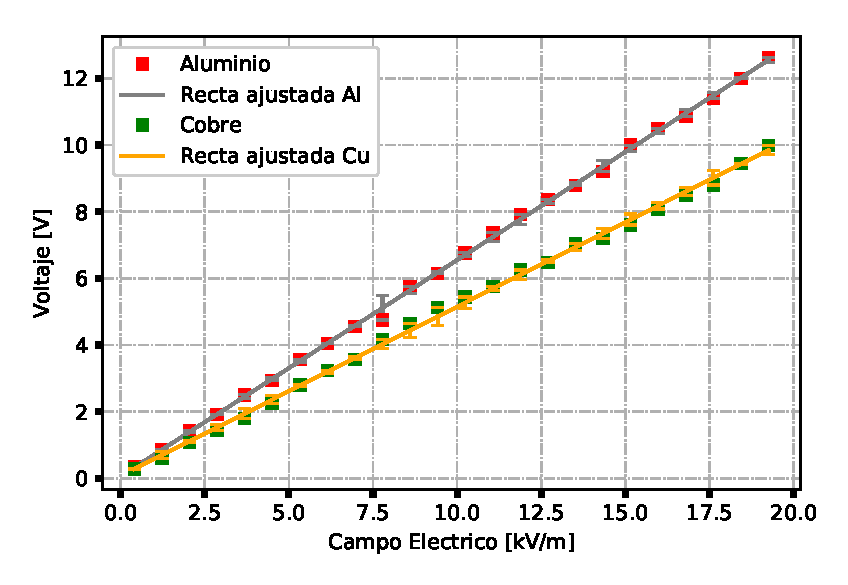
\includegraphics[width=0.8\textwidth]{Figures/Al_vs_Cu.eps}
\caption[Gráfica del voltaje inducido para distintos materiales]{Gráfica del voltaje inducido en un sensor emill con electrodo de cobre (verde) y un sensor emill con electrodo de aluminio (rojo). Ambos electrodos de 62 mm de diámetro, el motor girando a 87 Hz y un campo eléctrico constante incidente de 16 kV/m.}
\label{alcu}
\end{center}
\end{figure}
Los resultados se encuentran en la Fig. \ref{alcu}, en donde se observa que el aluminio posee mejor respuesta, sin embargo considerando la complejidad que conlleva trabajar con este material y haciendo notar que la diferencia en las respuestas es menor al 20\%, se opta por trabajar con cobre.\\

Para seleccionar la velocidad de giro óptima se realizaron pruebas de laboratorio variando la velocidad del motor y observando el voltaje inducido en las placas del sensor, los resultados de las pruebas arrojaron los resultados que se observan en la Fig. \ref{fv}.
\begin{figure}[h!]
\begin{center}
\includegraphics[width=0.8\textwidth]{Figures/Frec_vs_Vind.eps}
\caption{Gráfica del voltaje inducido vs la frecuencia de giro del motor para un campo eléctrico constante de 16 kV/m.}
\label{fv}
\end{center}
\end{figure}
Ya que el motor tenía un límite de 9 V en la alimentación definido por el fabricante, se estableció un rango de frecuencias de 100 Hz a 600 Hz. Para seleccionar la velocidad adecuada para el motor se tuvieron en cuenta el consumo de energía, la vibración y el ruido auditivo,  por lo que se decidió trabajar con un frecuencia de giro de 87 Hz, obteniéndose una señal sinusoidal de 260 Hz aproximadamente.

\subsection{Conversión corriente a tensión}
El movimiento del obturador permite la carga y descarga de la placa sensible, y en consecuencia, el área efectiva de la placa en la que se inducen cargas debido al campo eléctrico varía con el tiempo. Esta variación temporal de área genera una corriente eléctrica que fluye desde la placa sensitiva, tal como se observó en la Eq. \ref{Eq3}.\\

Debido a que la corriente que fluye desde la placa sensitiva es del orden de micro-amperios, es necesario implementar una topología que nos permita medirla, el circuito se muestra en la Fig. \ref{iv}. El circuito esta compuesto por un seguidor de voltaje tipo buffer y un divisor de tensión resistivo, los valores de resistencia se escogieron teniendo en cuenta el rango de medición del sensor. El voltaje en la resistencia R2 se mide con un seguidor de voltaje para acoplar impedancias entre el divisor y el circuito posterior de acondicionamiento.\\

\begin{figure}[h!]
\begin{center}
\includegraphics[width=.5\textwidth]{Figures/I-V.eps}
\caption{Circuito conversión corriente a tensión.}
\label{iv}
\end{center}
\end{figure}
El rango de medición del sensor se escogió teniendo en cuenta el valor de campo eléctrico mínimo que logra desencadenar un RREA (por sus siglas en inglés Relativistic Runaway Electron Avalanche), siendo este de aproximadamente 286 kV/m\cite{skeltved2017constraints}. La relación de ganancia del divisor de voltaje viene dado por la Eq. \ref{rel}, siendo R1 de 1 M$\Omega$ y R2 un potenciómetro de 500K que se establece en aproximadamente 80 k$\Omega$ con lo cual se consigue una relación de voltaje entrada-salida de aproximadamente $\frac{1}{15}$.
\begin{equation}
    \frac{Vin}{Vout}=\frac{R1}{R1+R2}=\frac{1}{15}
    \label{rel}
\end{equation}
Para simular el circuito \ref{iv}, se utilizó el programa LTspice de licencia abierta, la carga entregada por la placa sensora se recreó con una fuente de corriente, se estableció la relación de ganancia tal como se muestra en la Eq. \ref{rel}, los resultados se observan en la Fig. \ref{ivgraf}, en la gráfica se tienen dos ondas de diferente color, la onda naranja representa la señal de corriente que es del orden de micro-amperios, y la onda azul representa el voltaje a la salida de la etapa buffer.\\

\begin{figure}[h!]
\begin{center}
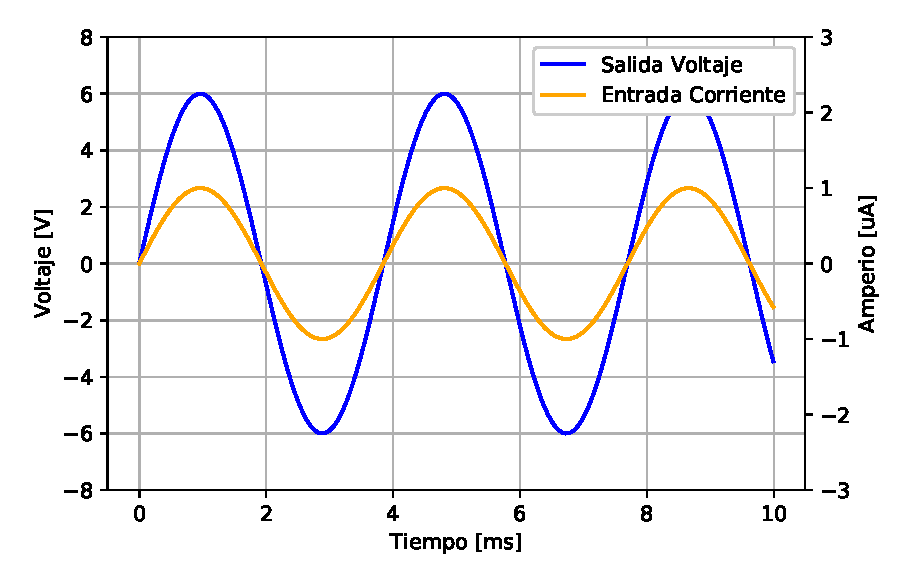
\includegraphics[width=0.8\textwidth]{Figures/I_V_graf.eps}
\caption[Gráfica de la simulación de la etapa corriente a tensión]{Gráfica obtenida de la simulación en LTspice del circuito \ref{iv}, la linea naranja representa la corriente que entrega la placa sensible, la azul es la onda de voltaje que se obtiene del divisor de resistivo, la atenuación del divisor resistivo aumenta el rango de medición en un factor de 15.}
\label{ivgraf}
\end{center}
\end{figure}

\subsection{Acondicionamiento de la señal}

Una de las propiedades más importantes del sensor de tipo molino, es que permite determinar la dirección del campo eléctrico vertical comparando la fase de giro del obturador y la fase de la señal que se induce en el plato sensible, para realizar esta comparación se utiliza el sistema embebido PSOC 5LP. Un PSOC (Programmable System on Chip) es un dispositivo fabricado por la empresa Cypress, esta conformado por microcontroladores cuya principal característica es contar con módulos tanto análogos como digitales en un solo chip, así mismo poder reconfigurar dinámicamente las entradas y salidas de estos módulos.\\

Para este proyecto se utilizó la tarjeta PSOC 5LP (ver Fig. \ref{psoc}), que cuenta con su propio kit de programación, procesador CPU ARM Cortex-M3, coprocesador DFB de hardware de 24 bits, opamps, PGA, filtros, comparadores, ADC SAR y Delta-Sigma y detección táctil CapSense. Las entradas analógicas del PSOC 5LP, manejan rangos de voltajes que van desde 0 V a 5 V, y la señal que se obtiene de la etapa de conversión corriente a tensión varia entre -12 V y 12 V, es por esto que se implemento un circuito de acondicionamiento (ver Fig. \ref{rs}), que reduce la amplitud y suma un nivel de DC a la señal de tal manera que se aproveche el rango de medición.\\

\begin{figure}[h!]
\begin{center}
\includegraphics[width=.8\textwidth]{Figures/psoc.png}
\caption[Kit programable PSOC 5LP]{Kit programable PSOC 5LP, conformado por microcontroladores cuya principal característica es contar  con módulos tanto análogos como digitales en un solo chip.}
\label{psoc}
\end{center}
\end{figure}

\begin{figure}[H]
\begin{center}
\includegraphics[width=.8\textwidth]{Figures/red_sum.eps}
\caption[Etapa de acondicionamiento de la señal]{Etapa de-amplificadora inversora de ganancia $1/5$, seguida de un restador de ganancia unitaria, que revierte la fase y le suma un nivel de offset.}
\label{rs}
\end{center}
\end{figure}

La etapa amplificadora inversora, relaciona el voltaje de entrada y salida por medio de la Eq. \ref{ganrs}, por lo que si se estable R4$>$R5, se puede de-amplificar la señal de entrada. Se escogió $R4=33\,k\Omega$ y $R5=6.8\,k\Omega$ para aprovechar el rango completo de los pines analógicos del PSOC, la ganancia que se obtiene es de $G=-\frac{1}{5}$, y en consecuencia, la señal a la entrada de la etapa se reduce a un rango entre -2.5 V y 2.5 V.
\begin{equation}
    V_{out}=-\frac{R_{5}}{R_{4}}V_{in}
    \label{ganrs}
\end{equation}
La etapa amplificadora inversora redujo la amplitud de la señal e invirtió la fase, por lo que en la siguiente etapa es necesario sumar un nivel de DC para cubrir el rango de medición de los pines analógicos e invertir nuevamente la fase de la señal, esto se logró mediante una etapa amplificadora restadora.
\begin{equation}
    Vout = \frac{R_{2}}{R_{1}}\left (V_{2}-V_{1} \right )
    \label{gres}
\end{equation}
En la Fig. \ref{rs}, se observa la topología y los valores de resistencias que se utilizaron para la etapa amplificadora restadora. Si $R6=R9$ y $R7=R8$ la relación entre la entrada y salida viene dada por la Eq. \ref{gres}, donde V1 es la señal que va a la entrada inversora y V2 a la entrada no inversora, el nivel de DC se escogió experimentalmente midiendo valores de campo eléctrico, se encontró que 2.225 V es el valor para el cual el campo eléctrico se aproxima a 0 V/m. En la Fig. \ref{rsgraf} encontramos los resultados de la simulación en LTspice del circuito de la Fig. \ref{rs}, donde la linea azul representa la señal que entrega la etapa de conversión corriente a tensión, y en naranja la señal después de aplicar la etapa de acondicionamiento, que redujo 5 veces la señal de entrada y sumo un nivel de DC de 2.225 V. 

\begin{figure}[H]
\begin{center}
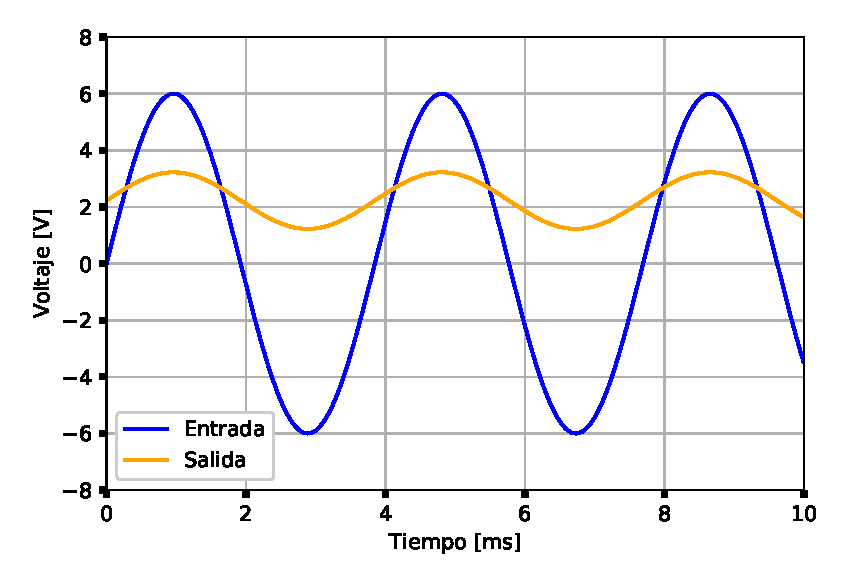
\includegraphics[width=.8\textwidth]{Figures/red_sum_graf.eps}
\caption[Simulación de la etapa de acondicionamiento de la señal]{Gráfica obtenidas de la simulación en LTspice del circuito  de la Fig. \ref{rs}, donde la linea azul representa la señal que entrega la etapa de conversión corriente a tensión, y en naranja la señal después de aplicar la etapa de acondicionamiento, que redujo 5 veces la señal de entrada y sumó un nivel de DC de 2.225 V}
\label{rsgraf}
\end{center}
\end{figure}
Los resultados de la implementación de la etapa de acondicionamiento se muestran en la Fig. \ref{acondicionamiento}, donde se observa la señal inducida en el sensor (azul), que corresponde a un campo eléctrico de 50 kV/m y la señal que se obtiene a la salida de la etapa de acondicionamiento (amarilla), la cual posee un nivel de DC de 2.35 V y se a reducido en un factor de $\sim$6.\\

\begin{figure}[H]
\begin{center}
\includegraphics[width=.8\textwidth]{Figures/Adec_signal.PNG}
\caption[Mediciones realizadas a la salida y entrada de la etapa de acondicionamiento]{Resultados de la implementación de la etapa de acondicionamiento, donde se observa la señal inducida en el sensor (azul), que corresponde a un campo eléctrico de 50 kV/m y la señal que se obtiene a la salida de la etapa de acondicionamiento (amarilla), la cual posee un nivel de DC de 2.35 V y se a reducido en un factor de $\sim$6.}
\label{acondicionamiento}
\end{center}
\end{figure}
\subsection{Etapa rectificadora de precisión}
% README: Explicación de la etapa, esquema del circuito, PSOC, primeras mediciones.
Con el fin de obtener una señal de DC que sea proporcional a las variaciones de campo eléctrico atmosférico, se implementó una etapa rectificadora de precisión utilizando el sistema embebido PSOC 5LP, el cual cuenta con el módulo MIXER (ver Fig. \ref{modulo}) que permite aplicar la operación de rectificación tomando como parámetros la señal que se obtiene de la etapa de acondicionamiento, la señal de la fase de giro del obturador la cual es medida con un encoder (EE-SJ3) y un voltaje de referencia que le indica al módulo en que nivel de offset aplicar la operación.\\

\begin{figure}[h!]
 \centering
  \subfloat[]{
   \label{modulo}
    \includegraphics[width=0.35\textwidth]{Figures/rect.eps}}
  \subfloat[]{
   \label{config_modulo}
    \includegraphics[width=0.65\textwidth]{Figures/mixer_config.PNG}}
 \caption[Módulo MIXER PSOC 5LP]{(a) Esquema del módulo MIXER, el cual tiene como entradas, la señal que entrega la etapa de acondicionamiento, la fase de giro del obturador medida con un encoder y un nivel de DC que establece el voltaje de operación del módulo. (b) Configuración del módulo hecha en el software de desarrollo PSOC Creator.}
 \label{mixer}
\end{figure}
El módulo MIXER hace parte de un conjunto amplio de librerías que se encuentra disponibles en el software PSOC Creator en su versión 4.2 libre de la empresa Cypress. En la Fig. \ref{config_modulo} se observa la configuración del módulo, se estableció la frecuencia de entrada de la señal en 300 Hz debido a que el módulo opera sobre un rango de frecuencia que va desde 0 Hz hasta el valor de frecuencia que se establece en el parámetro, también se escogió reloj externo ya que de esta forma podemos definir la señal que se obtiene del encoder que corresponde al la fase de giro del obturador como el reloj del módulo.

\begin{figure}[h!]
\begin{center}
\includegraphics[width=.8\textwidth]{Figures/rect_pos.eps}
\caption[Operación del módulo MIXER, con una señal en fase al giro del motor]{Gráfica de la operación del módulo MIXER, la señal azul representa la salida de la etapa de acondicionamiento, la señal verde es la salida del encoder y la señal amarilla es el voltaje de salida del módulo. Cada vez que el encoder envía un 0 lógico, la señal es rectificada, lo que causa un aumento del valor medio de la señal respecto al valor de referencia.}
\label{psgraf}
\end{center}
\end{figure}
El encoder envía una señal cuadrada digital de 1 o 0, que tiene la misma frecuencia de la señal del sensor y esta en fase con el giro del obturador. El modulo MIXER, invierte la señal cada vez que el encoder envía un 0 lógico, la señal que se obtiene es la misma que en un rectificador de media onda, en el caso en el que la señal que entrega la etapa de acondicionamiento se encuentre en fase con la señal que se obtiene del encoder, va a rectificar únicamente los lóbulos negativos, lo que va a causar un aumento en el valor promedio  respecto al valor de referencia, tal como se observa en la Fig. \ref{psgraf}.\\

En el caso de que la señal de la etapa de acondicionamiento este desfasada 180 grados respecto a la señal del encoder, el modulo va a rectificar únicamente los lóbulos positivos de la señal, lo que va a causar una disminución del valor promedio respecto al valor de referencia, tal como se observa en la Fig. \ref{pngraf}.\\

\begin{figure}[H]
\begin{center}
\includegraphics[width=.8\textwidth]{Figures/rect_neg.eps}
\caption[Operación del módulo MIXER, con una señal en desfase al giro del motor]{Gráfica de la operación del módulo MIXER, la señal azul representa la salida de la etapa de acondicionamiento, la señal verde es la salida del encoder y la señal amarilla es el voltaje de salida del módulo. cada vez que el encoder envía un 0 lógico, la señal es rectificada, lo que causa una disminución del valor medio de la señal respecto al valor de referencia.}
\label{pngraf}
\end{center}
\end{figure}
 

\begin{figure}[H]
\begin{center}
\includegraphics[width=.8\textwidth]{Figures/ope_psoc.PNG}
\caption[Medición de las señales de la etapa de rectificación]{Medición de la operación del módulo MIXER, el cual utiliza la señal del encoder (roja) para aplicar una rectificación (amarilla) sobre la señal proveniente de la etapa de acondicionamiento (azul), esta rectificación se hace de acuerdo a la fase de la señal azul. Cada vez que el encoder envía un 0 lógico, la señal es rectificada, lo que causa un aumento del valor medio de la señal respecto al valor de referencia.} 
\label{rect_real}
\end{center}
\end{figure}
En la Fig. \ref{rect_real} se observa la medición de la operación del módulo MIXER, el cual rectifica la señal de la etapa de acondicionamiento, de acuerdo a la fase medida mediante un encoder (azul), obteniéndose una señal rectificada (amarilla) proporcional al campo eléctrico.\\


\subsection{Filtro pasa bajas}
% README: Todo lo referente al filtro
La onda obtenida del rectificador de precisión posee un rizado proporcional a la magnitud del campo eléctrico medido, este rizado se elimina mediante un filtro pasabaja pasivo (en cascada al circuito). En este proyecto se utilizó un capacitor de 400 $\mu$F el cual elimina completamente el rizado de la señal, posee un tiempo de establecimiento de aproximadamente 400 s y su frecuencia de corte es de 400 $\mu$Hz, esto significa que unicamente permite las componentes de DC, tal como se observa en el diagrama de bode de la Fig. \ref{bode}.\\

\begin{figure}[h!]
 \centering
  \subfloat[]{
   \label{cap}
    \includegraphics[width=0.2\textwidth]{Figures/filtro.eps}}
  \subfloat[]{
   \label{bode}
    \includegraphics[width=0.65\textwidth]{Figures/bode.eps}}
 \caption[Filtro pasabajas]{(a) Circuito filtro capacitivo, el cual permite eliminar el rizado de la señal proveniente de la etapa rectificadora. (b) Diagrama de bode del filtro capacitivo, su frecuencia de corte es de alrededor de 400 $\mu$Hz, lo que significa que permite únicamente el paso de la componente en DC.}
 \label{bajas}
\end{figure}
La señal que se obtiene al aplicar el filtro capacitivo, es una señal de DC proporcional al campo eléctrico atmosférico, esta señal de Dc tiene un rango de operación entre 0 V y 5 V. En la Fig. \ref{pbgraf} se observa la onda proveniente de la etapa rectificadora (azul) y la señal de DC (amarilla) que se obtiene al aplicar el filtro capacitivo en cascada.\\

\begin{figure}[h!]
\begin{center}
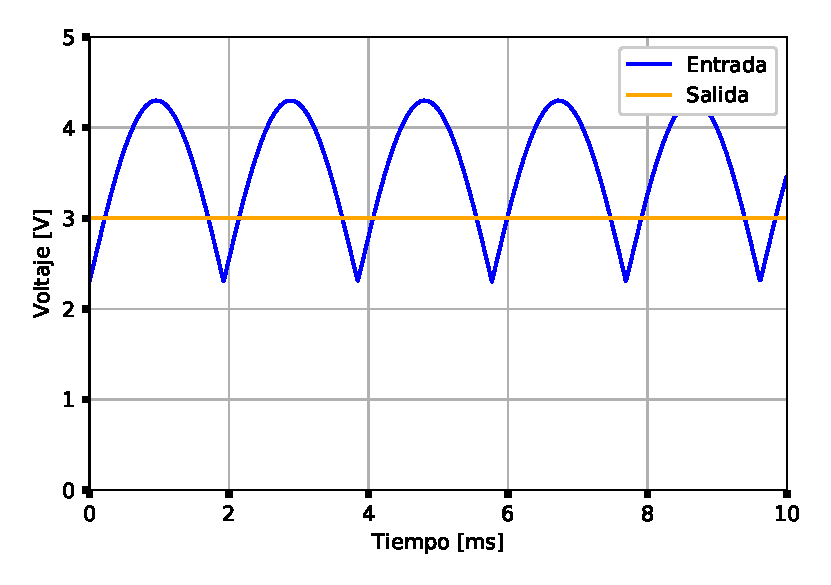
\includegraphics[width=.8\textwidth]{Figures/filtro_graf.eps}
\caption[Simulación del filtro pasabajas]{La señal de entrada corresponde a la señal que entrega la etapa rectificadora (azul), al aplicar el filtro capacitivo se obtiene una señal continua (amarilla) que es proporcional al campo eléctrico.}
\label{pbgraf}
\end{center}
\end{figure}

\subsection{Digitalización}
% README: ADC PSOC y sus caracterizticas
Uno de los objetivos de la estación es transmitir los datos utilizando protocolo I$^{2}$C, por lo que fue necesario digitalizar la señal de DC proporcional al campo eléctrico atmosférico que se obtuvo en la etapa del filtro pasabaja.

\begin{figure}[H]
 \centering
  \subfloat[]{
   \label{p1}
    \includegraphics[width=0.3\textwidth]{Figures/digitalizacion.eps}}
  \subfloat[]{
   \label{p2}
    \includegraphics[width=0.55\textwidth]{Figures/adc_config.PNG}}
 \caption[Módulo ADC SAR del PSOC 5LP]{(a) Digitalización de la señal de CC, con un ADC de tipo SAR, embebido en la tarjeta PSOC 5 LP . (b) Configuración del modulo ADC de la tarjeta PSOC 5LP.}
 \label{adc_muestreo}
\end{figure}
La digitalización de la señal, se hizo con un ADC delta-sigma de 20 bits el cual esta embebido en la tarjeta PSOC 5LP. En la Fig. \ref{adc_muestreo} se muestra el módulo del ADC y sus parámetros de configuración, los cuales se puede encontrar en las librerías del programa PSOC Creator en su versión 4.2. Para la configuración del módulo se seleccionó entrada tipo (Single ended) de 20 bits, frecuencia de muestreo de 183 SPS, rango de entrada de Vssa a Vdda, modo de conversión continuo, modo rail to rail del buffer y voltaje de referencia de Vdda/4.\\

\begin{figure}[h!]
\begin{center}
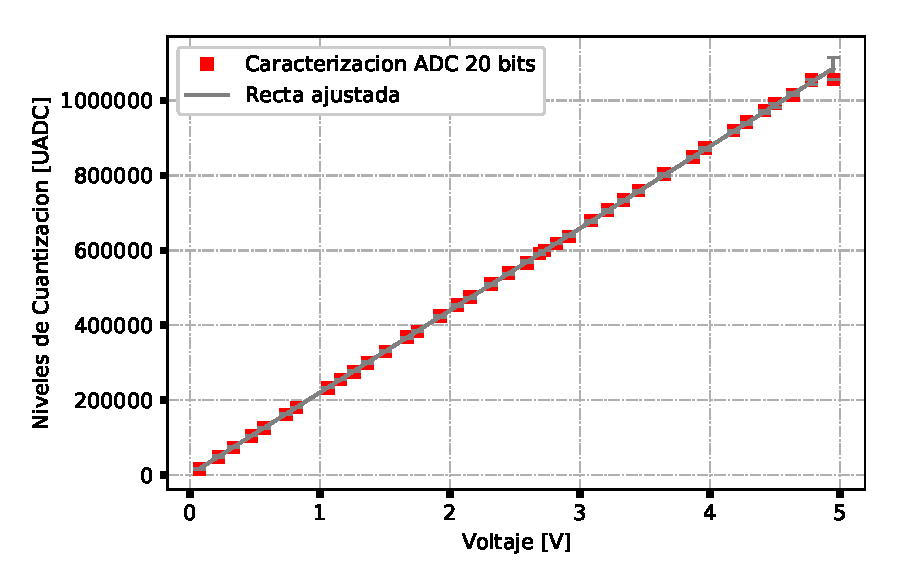
\includegraphics[width=0.8\textwidth]{Figures/ADC.eps}
\caption[Calibración del ADC SAR del PSOC 5LP]{Calibración del ADC tipo SAR embebido en la tarjeta PSOC 5LP, donde podemos observar que 1 UADC equivale a aproximadamente 4,5 $\mu$V}%CYPRESS   
\label{adc_curve}
\end{center}
\end{figure}
La caracterización del ADC se realizó aplicando un voltaje en su entrada y observando el valor de conversión medido. En la Fig. \ref{adc_curve} se muestra la gráfica de la calibración que se obtuvo, en donde podemos observar que 1 UADC equivale a aproximadamente 4,5 $\mu$V.


\subsection{Transmisión de datos}
% README: Transmisión i2c con el 
La transmisión se hizo con la tarjeta PSOC 5LP que cuenta con un módulo I$^{2}$C. En la Fig. \ref{transmision} se encuentra el módulo EZI2C y sus parámetros de configuración, se seleccionó una velocidad de transmisión de 100 kbps, una dirección esclava y pines conexión predeterminados. Para implementar el módulo se utilizó un código en lenguaje de programación C (ver Anexo \ref{adc_i2c}), el cual inicializa el módulo, define la dirección del módulo en 0x60 y finalmente transmite los valores que se le asignan al buffer donde se almacenan los datos medidos por el ADC.\\

\begin{figure}[h!]
 \centering
  \subfloat[]{
   \label{tra1}
    \includegraphics[width=0.35\textwidth]{Figures/transmicion.eps}}
  \subfloat[]{
   \label{tra2}
    \includegraphics[width=0.65\textwidth]{Figures/i2c_config.PNG}}
 \caption[Módulo I2C del PSOC 5LP]{(a) Transmisión de los valores en memoria mediante el módulo I$^{2}$C, embebido en la tarjeta PSOC 5 LP . (b) Configuración del módulo I$^{2}$C.}
 \label{transmision}
\end{figure}
En la Fig. \ref{i2c_pines} se encuentra los pines del PSOC 5LP utilizados por el sensor de campo eléctrico. Se definieron los pines P12[1] (sda) y P12[0] (scl) para la transmisión I$^{2}$C.

\begin{figure}[h!]
\begin{center}
\includegraphics[width=0.8\textwidth]{Figures/pines.png}
\caption{Pines utilizados por la tarjeta PSOC 5LP}
\label{i2c_pines}
\end{center}
\end{figure}
Se digitalizó una señal triangular utilizando el ADC tipo SAR y se transmitió vía I$^{2}$C. En los resultados se encontró que los datos recibidos tenían errores. Estos errores se debían a que mientras que el ADC guarda el valor digitalizado en memoria, el I$^{2}$C intenta leerlo, causando un error de lectura, por lo que se puso un tiempo de espera en la transmisión de 100 ms, para dar tiempo al ADC de registrar los valores medidos. 

\section{Calibración}
% README: Generador de campo eléctrico controlado y calibración hecha.
\subsection{Caracterización del generador de campo }
La calibración del sensor de campo eléctrico lento, se realizó utilizando un generador de campo controlado. Dicho generador está compuesto por un capacitor cuadrado de placas paralelas de 20 cm x 20 cm de área y 10 cm de separación, cuya capacitancia es de 3.54 $p$F. En la Fig. \ref{cap} se observa un esquema del montaje, se utilizaron tubos de PBC para separar y aislar eléctricamente los platos de baquela, la cual posee un recubrimiento de cobre de 35 $\mu$m.\\

\begin{figure}[h!]
\begin{center}
\includegraphics[width=0.8\textwidth]{Figures/calibracion_esquema.eps}
\caption[Esquema de los platos del generador de campo eléctrico controlado]{Fuente de campo eléctrico controlado que genera de 0 V/m a 20 kV/m, por medio de una fuente programable de alto voltaje DC/DC EMCO C20.}
\label{cap}
\end{center}
\end{figure}
Para el proceso de calibración se tuvo en cuenta la metodología propuesta por Cui et. al. \cite{cui2017model}, que establece el proceso a seguir para la calibración del sensor de campo eléctrico tipo molino, utilizando un capacitor de placas paralelas que genera un campo eléctrico controlado. El campo producido por un capacitor de placas paralelas se puede describir por la expresión de la Eq. \ref{campo}.
\begin{equation}
     E = \frac{V}{d}
     \label{campo}
\end{equation}
Donde E es el campo eléctrico, V es el voltaje entre las placas y d la distancia de separación. Se estableció una distancia fija de 10 cm, con el fin de controlar el valor del campo inducido entre las placas, regulando el voltaje aplicado. En este caso se utilizó una fuente DC/DC EMCO C20 programable de alta precisión. El control del generador de campo se hace mediante una señal de 0 a 5 V (Vctrl), lo que produce en la fuente DC/DC un voltaje de salida de 0 a 2 kV y en el capacitor de placas paralelas campos eléctricos entre 0 y 20 kV/m.\\

\begin{figure}[h!]
\begin{center}
\includegraphics[width=0.89\textwidth]{Figures/Esq_Ectrl.eps}
\caption[Esquema general del generador de campo eléctrico controlado]{Esquema general del generador de campo eléctrico, se utiliza una interfaz en Python programada en un Raspberry Pi para configurar los valores de voltaje de control vía ethernet desde un servidor, la fuente EMCO C20 genera voltajes entre 0 y 2 kV lo que establece un campo eléctrico entre la placas en un rango de 0 a 20 kV/m.}
\label{esq_ectrl}
\end{center}
\end{figure}
En la Fig. \ref{esq_ectrl} se muestra el esquema del banco de prueba implementado para el proceso de calibración. Mediante una interfaz creada en Python se configura el campo eléctrico aplicado a las placas del capacitor. Para ello se utiliza el DAC MCP4725 de 12 bits obteniéndose una resolución de $\sim$5 V/m. El DAC es controlado por una interfaz I$^{2}$C desde una Raspberry Pi conectada vía ethernet a un servidor.\\

\begin{figure}[H]
\begin{center}
\includegraphics[width=0.80\textwidth]{Figures/Fuente_E.eps}
\caption{Calibración del generador de campo eléctrico programable.}
\label{cal_fuente}
\end{center}
\end{figure}
Antes de calibrar el sensor de campo lento es necesario caracterizar el generador de campo eléctrico, para ello se aplicaron voltajes en un rango de 0 a 5 V con pasos de 0.1 V desde una interfaz en Python. Los resultado obtenidos se muestra en la Fig. \ref{cal_fuente}, donde se observa que la curva obtenida se ajusta a una recta que varia 4.095 V/m por cada mV en el Vctrl.

\subsection{Calibración del sensor}
referenciar la norma de calibración

IEEE Guide for the Measurement of DC Electric-Field Strength and Ion Related Quantities

y este artículo

Model, Design, and Testing of Field Mill Sensors for Measuring Electric Fields Under High-Voltage Direct-Current Power Lines, Yong Cui, 2018

Para la calibración del sensor de campo eléctrico lento, se ubicó el sensor entre las placas del capacitor tal como se muestra en la Fig. \ref{cap}, a continuación se generaron campos entre 0 y 20 kV/m con pasos de $\sim$400 V/m. Los resultados obtenido se muestran en la Fig. \ref{emill_graf}, donde se observa que la curva obtenida se ajusta a una recta que varía a razón de 90.6 mV por cada kV/m aplicado.

\begin{figure}[h!]
\begin{center}
\includegraphics[width=.85\textwidth]{Figures/Emill_Completo.eps}
\caption{Calibración del sensor de campo eléctrico, bajo condiciones ideales.}
\label{emill_graf}
\end{center}
\end{figure}


\section{Primeras mediciones}
% REAME: Gráficas de las mediciones hechas por la estación, descripción del comportamiento del campo eléctrico.
El prototipo de sensor de campo eléctrico, se instaló en una plataforma elevada a 3 m del suelo, con una estructura en tubos de PVC, ya que estos se construyen para resistir la intemperie, la estructura es modular, tal como se observa en la Fig. \ref{estructura}. El sensor se ubica de forma vertical en el extremo de la estructura, por lo que los platos quedan invertidos, esto se considera a la hora de interpretar, los datos registrados.\\

\begin{figure}[H]
 \centering
  \subfloat[]{
   \label{real_estr}
    \includegraphics[width=0.5\textwidth]{Figures/estructura.jpeg}}
  \subfloat[]{
   \label{esq_estr}
    \includegraphics[width=0.5\textwidth]{Figures/estructura.eps}}
 \caption[Estructura mecánica del sensor de campo lento]{(a) Estructura mecánica hecha en PVC, que soporta al sensor de campo eléctrico lento. (b) Esquema de la estructura mecánica del sensor de campo eléctrico lento, con sus respectivas dimensiones.}
 \label{estructura}
\end{figure}
Las primeras mediciones del sensor captaron se realizaron los días 08, 09 y 10 de Noviembre del año 2019 en la ciudad de Bucaramanga, Santander en el observatorio del grupo Halley de la Universidad Industrial de Santander. En la Fig. \ref{med} se puede observar los datos del campo eléctrico registrado. Xu B. et. al. encontraron que el campo eléctrico diurno en condiciones normales (fairweather), varía entre 50 y 220 V/m \cite{xu2013periodic}, lo cual concuerda con las mediciones realizadas por el prototipo.\\

\begin{figure}[h!]
\begin{center}
\includegraphics[width=0.8\textwidth]{Figures/mediciones.eps}
\caption[Registro de las primeras mediciones realizadas con el sensor]{Registro de campo eléctrico atmosférico hechas con el primer prototipo de sensor tipo molino los días 08, 09 y 10 de Noviembre del año 2019, donde se resalta el campo eléctrico en un día con condiciones normales, campo eléctrico nocturno y los eventos registrados para un día de tormenta.}
\label{med}
\end{center}
\end{figure}
El campo eléctrico nocturno durante los días de registro mostraba un aumento debido a la acumulación de nubes sobre el sensor por la disminución de temperatura ambiente. En una tormenta eléctrica el campo eléctrico atmosférico varía debido a descargas atmosféricas y acumulación de carga en las nubes \cite{xu2013periodic}. En la Fig. \ref{tormenta} se observa el comportamiento del campo eléctrico atmosférico el día 09 de Noviembre del año 2019 entre las 3 am y 5 am en la ciudad de Bucaramanga, en donde se presentaron precipitaciones y tormentas eléctricas. 

\begin{figure}[h!]
\begin{center}
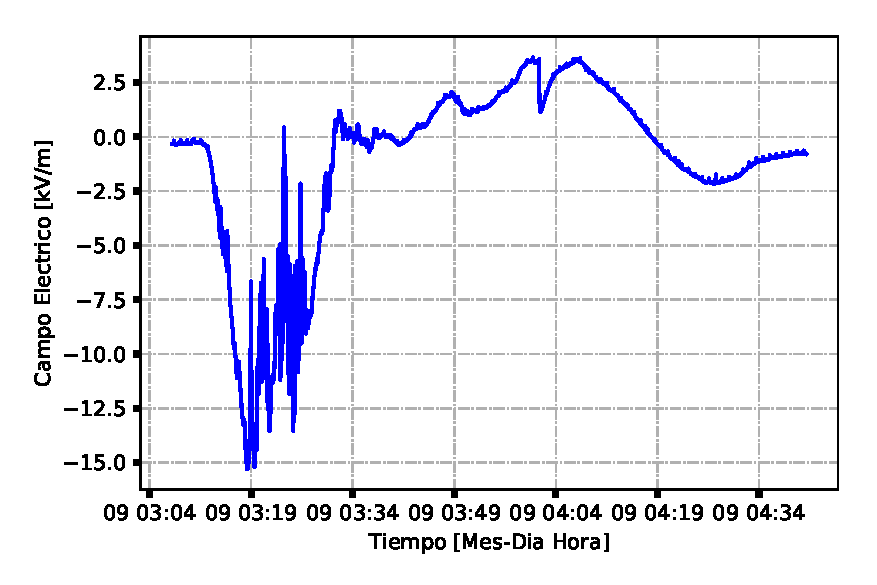
\includegraphics[width=0.8\textwidth]{Figures/tormenta.eps}
\caption[Registro de las primeras mediciones de tormentas eléctricas]{Registro de campo eléctrico atmosférico hechas con el primer prototipo de sensor tipo molino el día 09 de Noviembre del año 2019 entre las 3 am y 5 am en la ciudad de Bucaramanga, en donde ocurrieron algunas tormentas eléctricas.}
\label{tormenta}
\end{center}
\end{figure}


\chapter{Campo eléctrico atmosférico rápido}
\label{ch:background}



\begin{figure}[h!]
\begin{center}
\includegraphics[width=0.85\textwidth]{Figures/Diagrama_Rodilla.PNG}
\caption{Espectro de  rayos cósmicos diferencial en función de la energía. Se puede observar también los diferentes rangos de medición de los principales observatorios. Tomado de \cite{mollerach2018progress}}
\label{Diagrama_Rodilla}
\end{center}
\end{figure}


\section{Características de $\vec{E}$ rápido }
\section{Métodos de detección}
\section{Diseño del sensor de $\vec{E}$ rápido}
\subsection{Antena}
\subsection{Acondicionamiento de señal}

circuito de integración

Compensation of integrator time constants for electric field
measurements. Kohlmann. Leer y citar

respuesta en frecuencia del integrador


\subsection{Digitalización}
\subsection{Sistema de lectura}
FPGA, Memoria


\begin{figure}[h!]
\begin{center}
\includegraphics[width=1\textwidth]{Figures/VHDL.eps}
\caption[Estructura de un espectroscopio]{El electroscopio contiene en su interior 2 láminas delgadas de un conductor, éstas a su vez están conectadas a una varilla conductora con una esfera al final o parte plana. Cuando la esfera interactúa con una superficie cargada, las 2 láminas adquieren la misma carga de la varilla y por lo tanto se repelen, indicando la presencia de una carga. Imagen tomada de \cite{gordon1883physical}}
\label{ELectroscopio}
\end{center}
\end{figure}

\subsection{Trasmisión de datos}

Resumen características:

\begin{table}[ht]
\centering
  \caption{ Frontend and readout parameters}
  \begin{tabular}{ | c | c |}
    \hline
    Parameter & Value\\ \hline
    antenna  type & flat\\ \hline
    diameter [cm] & 20  \\ \hline
    recording length [ms] &  1000 \\ \hline
    pre-trigger [ms] & 200 \\ \hline
    post-trigger [ms] & 800 \\ \hline
    sampling frequency [Mhz] & 1 \\ \hline
    digitazion resolution [bits] & 12 \\ 
    \hline
  \end{tabular}
  \label{net}
\end{table}
Ref. Types of lightning discharges that abruptly terminate enhanced fluxes of energetic radiation and particles observed at ground level. Chilingarian. 2017


\section{Calibración}
\section{Primeras Mediciones}
\chapter{Estación de monitoreo de campo eléctrico}
\label{ch:background}

La estación tiene como fin observar, medir, codificar y transmitir las variables atmosféricas que apoyen el estudio de los mecanismos de aceleración de partículas secundarias cargadas. El campo eléctrico atmosférico es la variable más relevante, sin embargo la medición de parámetros como temperatura, humedad y presión permite ampliar el estudio de los fenómenos y eventos relacionados a la generación de campo eléctrico atmosférico, como la altura de la nube, el potencial eléctrico atmosférico y ubicación geográfica de las descargas atmosféricas.

\section{Variables atmosféricas}
Desde la formación de nubes de tormenta hasta la disipación de las misma encontramos algunas variables atmosféricas que nos ayudan a entender los eventos que ocurrieron durante el desarrollo de una tormenta eléctrica e incluso nos permiten predecirlas. La importancia de este proyecto radica en la capacidad de medir el campo eléctrico atmosférico y algunas las variables relacionadas, como la altura de la nube y potencial eléctrico, también resulta de gran relevancia conocer la ubicación de las descargas atmosféricas que producen campos eléctricos transitorios y en general, como se mencionó anteriormente, ayudar al estudio de los mecanismos de aceleración de partículas secundarias cargadas.
\subsection{Temperatura}
El calentamiento de la atmósfera es el resultado del balance entre la radiación entrante y saliente de la superficie terrestre. La mayor parte de la radiación solar incidente es absorbida por la parte superficial del suelo y como consecuencia se torna más caliente que el aire que está en contacto directamente con ella. Por la noche, una cantidad considerable de calor se irradia desde la superficie del suelo y causa un enfriamiento en la parte más superficial del mismo \cite{jaramillo2005clima}.\\

Las corrientes de aire caliente a menudo son provocadas por la misma radiación térmica. Cuando se produce un choque entre un frente frió y una de estas corrientes de aire caliente, se produce una condensación de agua que desemboca con frecuencia en una nube de tormenta, es por esto que se considera relevante para el estudio de la formación de tormentas eléctricas.\\

Para medir la temperatura del aire se utilizó un sensor BME280, voltaje de alimentación entre 1.71 V y 3.6 V, consume 3.6 $\mu$A para un periodo de muestreo de 1 Hz, rango de operación entre -40 $^{\circ}C$ y +85 $^{\circ}C$, posee una resolución de $\pm$0.5 $^{\circ}C$, utiliza I$^{2}$C y SPI como protocolos de transmisión de datos, en la Fig. \ref{bme_t} se muestra el sensor comercial fabricado por la empresa Sparkfun, junto a su tabla de especificaciones tomada del datasheet.

\begin{figure}[h!]
 \centering
  \subfloat[]{
   \label{t1}
    \includegraphics[width=0.25\textwidth]{Figures/bme.jpg}}
  \subfloat[]{
   \label{t2}
    \includegraphics[width=0.75\textwidth]{Figures/bme_tem.PNG}}
 \caption{(a) Sensor BME280 humedad, presión y temperatura. (b) Tabla de especificaciones del sensor, el cual tiene un voltaje de alimentación entre 1.71 V y 3.6 V, consume 3.6 $\mu$A para un periodo de muestreo de 1 Hz, rango de operación entre -40 $^{\circ}C$ y +85 $^{\circ}C$, posee una resolución de $\pm$0.5 $^{\circ}C$, utiliza I$^{2}$C y SPI como protocolos de transmisión de datos.}
 \label{bme_t}
\end{figure}

\subsection{Humedad}
Dentro de la atmósfera el agua puede estar presente como vapor de agua (un gas invisible), como gotas de agua y como cristales de hielo (fases visibles). El vapor de agua ingresa en la atmósfera por evaporación (desde el océano, ríos, lagos), transpiración desde las plantas y sublimación del hielo y la nieve. El vapor de agua es uno de los constituyentes del aire, se caracteriza por ser variable en cantidad, de acuerdo con la disponibilidad de agua y energía y representa hasta un 4$\%$ en volumen del aire. Este volumen es determinado por la temperatura del ambiente, a mayor temperatura del aire hay mayor capacidad de retención de humedad\cite{jaramillo2005clima}.\\

La tormenta es la manifestación extrema de la inestabilidad atmosférica. Se produce con el cumulonimbus y va acompañada de un cierto número de fenómenos tales como descargas atmosféricas  y lluvias. Los requisitos iniciales para la formación del cumulonimbus que desemboca en tormenta, es la presencias de aire húmedo, un gradiente vertical de temperatura y un fuerte mecanismo de elevación para forzar el aire hacia arriba. Cuanto mayores son las diferencias de densidad entre las masas de aire (temperatura y humedad), mayores son las inestabilidades atmosféricas que se desarrollan y mayor es la intensidad de estas tormentas \cite{price2009thunderstorms}.\\

\begin{figure}[H]
 \centering
  \subfloat[]{
   \label{h1}
    \includegraphics[width=0.25\textwidth]{Figures/bme_2.jpg}}
  \subfloat[]{
   \label{h2}
    \includegraphics[width=0.7 \textwidth]{Figures/bme_hum.PNG}}
 \caption{(a) Sensor BME280 humedad, presión y temperatura. (b) Tabla de especificaciones del sensor, su voltaje de alimentación esta entre 1.71 V y 3.6 V, consume 3.6 $\mu$A para un periodo de muestreo de 1 Hz, rango de operación entre 0 $\%$RH y 100 $\%$RH, posee una resolución de $\pm$0.008 $\%$RH, con una tolerancia de $\pm$3 $\%$RH, utiliza I$^{2}$C y SPI como protocolos de transmisión de datos.}
 \label{bme_h}
\end{figure}

Se seleccionó el sensor BME280 para las mediciones de humedad, su voltaje de alimentación esta entre 1.71 V y 3.6 V, consume 3.6 $\mu$A para un periodo de muestreo de 1 Hz, rango de operación entre 0 $\%$RH y 100 $\%$RH, posee una resolución de $\pm$0.008 $\%$RH, con una tolerancia de $\pm$3 $\%$RH, utiliza I$^{2}$C y SPI como protocolos de transmisión de datos, en la Fig. \ref{bme_h} se muestra el sensor comercial fabricado por la empresa Sparkfun, junto a su tabla de especificaciones tomada del datasheet.\\

\subsection{Presión}
La presión atmosférica es la más empleada al estudiar la atmósfera y el aire, se define como el peso que ejerce el aire sobre la unidad de superficie. Se puede obtener una medida de la presión atmosférica en un lugar determinado pero de ella no se pueden sacar muchas conclusiones; sin embargo, la variación de dicha presión a lo largo del tiempo permite obtener una información útil que, unida a otros datos meteorológicos (temperatura atmosférica, humedad y vientos), puede dar una imagen bastante acertada del tiempo atmosférico en dicho lugar e incluso un pronóstico a corto plazo del mismo \cite{blanco1997programa}.\\

Cuando el aire está frío, se contrae, aumenta la densidad y, por lo tanto, desciende, haciendo aumentar la presión y provocando estabilidad barométrica o anticiclónica. Se forma así una zona de calmas, es decir, sin vientos, ya que el aire frío y pesado desciende lentamente en sentido circular y comienza a girar casi imperceptiblemente en sentido horario en el hemisferio norte y antihorario en el hemisferio sur. Se forma, entonces, un anticiclón. Cuando el aire está caliente, asciende, haciendo bajar la presión y provocando inestabilidad. Se forma así un ciclón o borrasca \cite{blanco1997programa}.\\

La presión atmosférica se mide en diferentes unidades. Entre ellas destacamos la atmósfera, el mm de Hg (mercurio) o tor y el milibar. La presión atmosférica normal es de 1.013 mb, pero ésta varía de un día a otro. Se seleccionó el sensor BME280 para las mediciones de presión, su voltaje de alimentación esta entre 1.71 V y 3.6 V, consume 3.6 $\mu$A para un periodo de muestreo de 1 Hz, rango de operación de 30,000 Pa a 110,000 Pa, posee una precisión relativa de 12 Pa y precisión absoluta de 100 Pa, utiliza I$^{2}$C y SPI como protocolos de transmisión de datos, en la Fig. \ref{bme_p} se muestra el sensor comercial fabricado por la empresa Sparkfun, junto a su tabla de especificaciones tomada del datasheet.\\

\begin{figure}[h!]
 \centering
  \subfloat[]{
   \label{p1}
    \includegraphics[width=0.25\textwidth]{Figures/bme_3.jpg}}
  \subfloat[]{
   \label{p2}
    \includegraphics[width=0.75\textwidth]{Figures/bme_press.PNG}}
 \caption{(a) Sensor BME280 humedad, presión y temperatura. (b) Tabla de especificaciones del sensor, su voltaje de alimentación esta entre 1.71 V y 3.6 V, consume 3.6 $\mu$A para un periodo de muestreo de 1 Hz, rango de operación de 30,000 Pa a 110,000 Pa, posee una precisión relativa de 12 Pa y precisión absoluta de 100 Pa, utiliza I$^{2}$C y SPI como protocolos de transmisión de datos.}
 \label{bme_p}
\end{figure}

\subsection{Altura de la nube y potencial eléctrico}
Sabemos que el campo eléctrico lento es producido por la acumulación de carga en las nubes, idealmente el conjunto atmósfera tierra se puede considerar como un capacitor esférico de placas paralelas, por lo que la expresión de la Eq. \ref{potencial} describe el comportamiento del potencial que se genera entre las nubes y la tierra, con $E$ como el campo eléctrico y $d$ la altura de la base de la nube cúmulo.
\begin{equation}
    V = Ed
    \label{potencial}
\end{equation}
G. Lawrence et. al. en su trabajo \textbf{"The Relationship between Relative Humidity and the Dewpoint Temperature in Moist Air"} \cite{lawrence2005relationship}, nos entrega una expresión para la aproximación de el nivel de condensación de elevación LCL, es decir, la altura de la base de la nube cúmulo ($Z_{lcl}$), que está estrechamente relacionado con la temperatura de rocío ($t_{d}$) y la temperatura del aire ($t$) a nivel de suelo tal como se observa en la Eq. \ref{alt}.
\begin{equation}
    Z_{lcl}\approx 125\left (t - t_{d}\right )
    \label{alt}
\end{equation}
La temperatura a la que se condensa (o solidifica) el vapor de agua en una muestra de gas a un valor de presión se le llama temperatura de punto de rocío ($t_{d}$) y su valor depende de la humedad relativa del gas ($RH$) \cite{lawrence2005relationship}, tal como se observa en la Eq. \ref{td}.
\begin{equation}
    td \approx t - \left ( \frac{100 - RH}{5}\right)
    \label{td}
\end{equation}

\section{Sistema de posicionamiento}
La estación de monitoreo, posee un sistema GPS que permite conocer el tiempo y ubicación de los eventos registrados, esto es importante para correlacionar eventos que ocurrieron en la misma franja temporal. El GPS utiliza los datos suministrados por al menos 4 satélites en orbita para conocer el tiempo y calcular su ubicación espacial.\\

El GPS que se utilizó en la estación es el Venus638FLPx de la compañía Sparkfun (ver Tabla. \ref{cara_gps}), por su tamaño, potencial y versatilidad, utiliza protocolo de comunicación serial a 9600 baudios, posee una velocidad de actualización de hasta 20 Hz con precisión de 2.5 m, se alimenta con 3.3 V y posee un pin para conexión de una batería externa o un supercondensador a la placa, para admitir reinicios rápidos después de desconectar la alimentación.\\

\begin{table}[]
\resizebox{\textwidth}{!}{%
\begin{tabular}{|c|c|}
\hline
\cellcolor[HTML]{FFFFC7}\textbf{CARACTERÍSTICAS} & \parbox{2cm}{\includegraphics[width=0.2\textwidth]{Figures/gps_venus.jpg}} \\ \hline
20 Hz de tasa de actualización & -148dBm  de sensibilidad de arranque en frío \\ \hline
Sensibilidad de seguimiento -165dBm & 29 segundos de arranque en frío TTFF \\ \hline
TTFF de 3,5 segundos con AGPS & 1 segundo arranque en caliente \\ \hline
Precisión de 2.5m & Detección y supresión de múltiples rutas \\ \hline
Detección y mitigación de atascos & Soporte SBAS (WAAS / EGNOS) \\ \hline
Efemérides extendidas de 7 días AGPS & Navegación a plena potencia de 67 mW \\ \hline
Funciona directamente con antena activa o pasiva & Flash interno para el registro opcional \\ \hline
Contiene LNA, filtro SAW, TCXO, RTC Xtal, LDO & Sin RoHS compatible con Pb \\ \hline
\end{tabular}%
}
\caption{Características del GPS Venus638FLPx de la compañía Sparkfun.}
\label{cara_gps}
\end{table}
El GPS suministra 6 tramas de datos llamadas NMEA, de las cual se puede obtener el tiempo, fecha, ubicación, cantidad de satélites, altitud entre otros. Las tramas que se analizan para el proyecto son la GGA (Global Positioning System Fix Data) y la RMC (Recommended Minimum Specific GNSS Data). De la trama GGA se obtiene una cadena de datos tal como se muestre en la Fig. \ref{GGA}, de donde se extrae el tiempo UTC (hhmmss.sss), latitud (ddmm.mmmm), indicador N/S (a), longitud (dddmm.mmmm), indicador E/W (a) y altitud (a).\\

\begin{figure}[H]
\begin{center}
\includegraphics[width=.8\textwidth]{Figures/GGA_RMC.png}
\caption[Trama de datos del GPS]{Trama de datos GGA y RMC suministrada por el GPS venus a una frecuencia de 1 Hz. De la trama GGA se obtiene el tiempo UTC (hhmmss.sss), latitud (ddmm.mmmm), indicador N/S (a), longitud (dddmm.mmmm), indicador E/W (a) y altitud (a), de la trama RMC se obtiene la fecha UTC (ddmmyy).}
\label{GGA}
\end{center}
\end{figure}
Existen varios métodos para determinar la ubicación de una descarga atmosférica, entre ellos tenemos técnicas de búsqueda de dirección (DF) \cite{krider1976gated}, tiempo de llegada (TOA) \cite{lee1989ground}, una combinación de estos dos \cite{cummins1998combined} y métodos de interferometría \cite{hayenga1981two}. Para el proyecto se utilizó una variación del método de tiempo de llegada (TOA), llamado algoritmo de trilateración el cual consiste en un método matemático para calcular un punto en el espacio usando distancias desde diferentes puntos de referencia a otras entidades geométricas conocidas, el número mínimo de entidades para poder aplicar el método es de 3, esto es tener una red espacialmente distribuida de mínimo 3 estaciones, la distancia se calcula midiendo el tiempo entre detección de cada estación de forma sincronizada, la diferencia entre los tiempos permite el cálculo de la ubicación de la descarga \cite{mialdea2019development}.\\

\begin{figure}[H]
\begin{center}
\includegraphics[width=.8\textwidth]{Figures/venus_esquema.png}
\caption[Esquema de conexión del GPS]{Esquema de conexión del GPS a un sistema de procesamiento que se encarga de extraer los datos, también se le coloca una batería de 3 V, con el fin de habilitar el arranque rápido del módulo.}
\label{ven_gps_esq}
\end{center}
\end{figure}
Para poder sincronizar cada una de las estaciones en la red, se utiliza la señal PPS suministrada por el GPS, el cual entrega un pulso digital de frecuencia 1 Hz y 4 ms en alto, la amplitud del pulso es de 3.3 V y permite realizar la sincronización temporal de las estaciones.En la Fig. \ref{ven_gps_esq} se muestra el esquema de conexión del GPS con el sistema de procesamiento central, que es el proyecto es una Raspberry pi 3 y una batería que permite el arranque rápido del dispositivo. Para el procesamiento de la trama de datos se utilizó un código en lenguaje Python, que extrae los datos requeridos de la trama principal (ver Anexo. \ref{gps_code}).

\section{Integración de periféricos}
La integración se hizo en torno a un sistema de procesamiento central el cual realiza la adquisición de los datos y posteriormente los almacenan. Para la estación se utilizó una Raspberry pi 3, la cual se encarga de la adquisición de los datos de cada uno de los sensores por medio de protocolos de comunicación como I2C o UART y posteriormente los almacena en una memoria SD, de tal manera que sea posible acceder a ellos mediante un servidor externo vía ethernet.\\

\begin{figure}[H]
\begin{center}
\includegraphics[width=.8\textwidth]{Figures/Esquema_racimo_storm.eps}
\caption[Esquema de conexión del sistema de adquisición de datos]{Esquema de conexión del sistema de adquisición de datos central que almacena los datos, los procesa y finalmente los carga a un servidor web en donde se podrán visualizar.}
\label{esq_racimo}
\end{center}
\end{figure}
Con el fin de recolectar los datos se crea un código de adquisición en lenguaje Python, el cual se encarga de la recolección y almacenamiento de los datos. En la Fig. \ref{esq_codigo} se muestra un diagrama de bloques del código, inicialmente se importan los módulos, se configuran y se crean la variables que se necesitan para el funcionamiento de los sensores, a continuación el algoritmo le pregunta al GPS la fecha y hora para posteriormente crear un archivo de texto con en el formato ``\textbf{Datos\_YYYY\_MM\_DD\_HH.txt}" donde (YYYY) es el año,  (MM) es el mes, (DD) el día y (HH) la hora, a continuación se realiza la adquisición de las variables temperatura, presión, humedad, campo eléctrico cada segundo y se almacenan en el archivo de texto que se creó, finalmente se pregunta si ha transcurrido una hora, con el fin de crear un nuevo archivo de texto nuevo o realizar nuevamente la adquisición de datos (Ver Anexo. \ref{}).\\

\begin{figure}[H]
\begin{center}
\includegraphics[width=.4\textwidth]{Figures/Esquema_codigo_racimo.eps}
\caption[Diagrama de bloques del código de adquisición]{Esquema de conexión del sistema de adquisición de datos central que almacena los datos, los procesa y finalmente los carga a un servidor web en donde se podrán visualizar.}
\label{esq_codigo}
\end{center}
\end{figure}

\subsection{Estructura mecánica}
Para la construcción de la estación de monitoreo se integró sensores de temperatura, humedad, presión, campo eléctrico rápido y lento, un sistema de posicionamiento global y un sistema de adquisición de datos. También se diseño una interfaz web en donde se visualizan los datos adquiridos por la estación. En la Fig. \ref{montaje} se muestra un esquema del montaje mecánico de la estación, compuesto por soportes para la antena de campo rápido, sensor de campo lento, sensor de temperatura, humedad y presión y una caja para la electrónica central.\\
\begin{figure}[H]
\begin{center}
\includegraphics[width=0.8\textwidth]{Figures/esquema_mecanico.eps}
\caption[Esquema de la estación de monitoreo de campo eléctrico]{Esquema del montaje mecánico de la estación de monitoreo de campo eléctrico, compuesto por una antena de campo rápido, un sensor de campo lento, un sensor de temperatura, humedad y presión y una caja de electrónica central.}
\label{montaje}
\end{center}
\end{figure}
\section{Interfaz de monitoreo}
\section{Primeras mediciones}
La estación de monitoreo se ubico sobre el laboratorio del grupo Halley de la Universidad Industrial de Santander y se puso adquirir desde el 1 de Noviembre de 2019 hasta mediados del mes de Diciembre del mismo año, durante este periodo ocurrieron varios eventos importantes sin embargo se resalta el que ocurrió el día 9 de Noviembre del 2019, debido a que la concentración de nubes de tormenta estaban sobre el sensor y fue posible captar el comportamiento del campo eléctrico. 
\begin{figure}[H]
\begin{center}
\includegraphics[width=0.8\textwidth]{Figures/Altura_nube.eps}
\caption{Primeras mediciones de altura de la base de la nube, para el día 9 de Noviembre del 2019, el sensor esta ubicado en el observatorio del grupo Halley de la Universidad Industrial de Santander.}
\label{temp}
\end{center}
\end{figure}
En base a las mediciones de temperatura y humedad se presentan en la Fig. \ref{temp}, las primeras valoraciones de altura de la base de la nube para un día lluvioso. Los datos se tomaron el día 9 de Noviembre del 2019, el sensor esta ubicado en el observatorio del grupo Halley de la Universidad Industrial de Santander. \\

\begin{figure}[H]
\begin{center}
\includegraphics[width=0.8\textwidth]{Figures/potencial.eps}
\caption{Primeras estimaciones del potencial atmosférico, para el día 9 de Noviembre del 2019, el sensor se ubicó en el observatorio del grupo Halley de la Universidad Industrial de Santander.}
\label{pot}
\end{center}
\end{figure}
Sus primeras estimaciones se hicieron en base a la Eq. \ref{potencial}, siendo $E$ el campo eléctrico medido con el sensor de campo lento, y $d$ la altura de la base de la nube. En la Fig. \ref{pot} se presentan la estimación del potencial eléctrico para el día 9 de Noviembre del 2019. Donde se observa la variación que 
  
%\input{State/State}
%\chapter{Metodología}

A continuación se describe detalladamente la metodología que se ha llevado a cabo para el cumplimiento de los objetivos del proyecto de investigación. En cada actividad también se describen los resultados preliminares obtenidos.

\section{Diseño y calibración del sistema electrónico del hodoscopio}

Para la medición del flujo de partículas dependiendo de la trayectoria se desarrollará un hodoscopio con dos paneles compuestos de 60 centelladores plásticos cada uno. Cada centellador tendrá un SiPM S13360-6050CS como elemento sensor. Las señales de cada panel serán discriminadas mediante un sistemas de adquisición (DAQ) basado en el Circuito de Aplicación Específica (ASIC) MAROC3A para luego ser almacenadas. El sistema DAQ es controlado por un computador embebido Rapsberry Pi. El hodoscopio tendrá un sistema de disparo estratificado que determinará la veracidad de los eventos detectados y las coincidencias entre los paneles que lo conforman. \\

Por otro lado, los SiPM serán caracterizados con el fin de determinar su comportamiento (ganancia y ruido) dependiendo de la temperatura y el voltaje de ruptura. La atenuación de la señal en las barras centelladoras será medida para diferentes puntos de interacción usando un sistema de estimulación controlado. Adicionalmente, se evaluará la respuesta de los paneles centelladores y el hodoscopio midiendo el flujo de muones atmosféricos en diferentes direcciones. Los resultados preliminares y detalles técnicos de las actividades relacionadas con este objetivo se muestran a continuación.\\


\textbf{Actividades y resultados preliminares}\\

\subsection{Diseño del hodoscopio}

El hodoscopio está formado por dos paneles sensibles compuestos de $30 \times 30$ barras centelladoras rectangulares de $120 \textrm{cm} \times 4 \textrm{cm} \times 1 \textrm{cm}$.\\

Los centelladores, fabricados por Fermilab, están hechos de poliestireno (Dow Styron $663$) con un recubrimiento externo de TiO$_2$ de 0.25 mm de espesor. Los dopantes del material primario son $1\%$ PPO  y $0.03 \%$ POPOP, con un pico máximo de emisión en 420 nm \cite{Anghel2015} y un tiempo de decaimiento de 1.6 ns \cite{Kleinknecht2005}. \\

Cada barra centelladora tiene un agujero de 1.8 mm de diámetro en su parte central donde va situada una fibra óptica de corrimiento de longitud de onda (WLS). En este caso se usa la fibra Saint-Gobain BCF-92 con un diámetro de 1.2 mm, un índice de refracción en el núcleo de 1.42, un pico de absorción de 410 nm y un pico de emisión de 492 nm \cite{Kuraray2018}.\\

En este caso se usa el SiPM Hamamatsu S13360-6050CS como elemento sensor. El SiPM tiene un área fotosensible de 
$1.3 \times 1.3 \textrm{mm}^2$, 667 píxeles, un factor de llenado 74$\%$, un voltaje de ruptura de 53$\pm$5 V (25 $^{\circ}$C), una ganancia de $10^5$ a $10^6$ y una eficiencia de foto-detección de  40$\%$ a 450 nm.\\

Los SiPM están acoplados de manera directa con la fibra óptica mediante un sistema mecánico anclado a la barra centelladora. Este sistema centra el extremo de la fibra óptica con la región sensible del SiPM. Ver Fig. \ref{SiPM_WLS}. Usualmente se utiliza resina óptica EJ200 de Eljen Technology para acoplar el SiPM y la fibra óptica, sin embargo, resultados de la simulación del centellador-fibra-SiPM en GEANT4 \cite{Vasquez2018} demuestran que su uso no aumenta el número de fotones que llegan al SiPM.

\begin{figure}[h!]
\begin{center}
\includegraphics[width=0.7\textwidth]{Figures/panel_frontend.png}
\caption{Sistema de acople entre la fibra WLS y el SiPM en cada barra centelladora.}
\label{SiPM_WLS}
\end{center}
\end{figure}

\subsection{Diseño de la electrónica del SiPM}

 La electrónica de acondicionamiento consta de una etapa de polarización del SiPM, una etapa de amplificación (con ganancia 94) y un acople de impedancias como se muestra en Fig. \ref{SiPM_Ele}. 
 
 El circuito de polarización alimenta el SiPM con un voltaje (HV) que varia entre 40V y 80V. La fuente HV se basa en el módulo controlable C11204 de Hamamatsu.
 
 \begin{figure}[h!]
\begin{center}
\includegraphics[width=0.7\textwidth]{Figures/Acondicionamiento.png}
\caption{Electrónica de polarización y acondicionamiento del SiPM.}
\label{SiPM_Ele}
\end{center}
\end{figure}

La fuente HV se basa en el módulo controlable C11204 de Hamamatsu el cual puede proporcionar voltajes entre 40V y 80V. Por otra parte, la amplificación de la señal pulsada se hace mediante el amplificador operacional OPA691 de Texas Instruments cuyo ancho de banda es 190 MHz. Finalmente, la señal amplificada se transmite a través de un cable coaxial RG178U con impedancia de 50 ohmnios y ancho de banda de 900 MHz.

\subsection{Diseño del sistema de adquisición del hodoscopio}

El sistema de adquisición se basa en el Circuito Integrado de Aplicación Específica (ASIC) MAROC3A de Omega, desarrollado para aplicaciones en detectores de partículas.

\begin{figure}[h!]
\centering
\includegraphics[scale=0.5]{Figures/Maroc.png}
\caption{Architectura del ASIC MAROC3A. La línea roja indica las etapas que recorre cada señal hasta su discriminación.}
\label{Maroc}
\end{figure}


La MAROC3A tiene 64 canales de lectura con una impedancia de entrada de 50 ohmios. Cada canal tiene una etapa de amplificación de ganancia programable (0-4), un \textrm{fast-shaper} unipolar con ganancia de 2.3V/pC y un discriminador (d1) con un umbral de discriminación ($V_{th0}$) establecido por un Convesor Digital-Análogo (DAC) de 10 bits (2.3 mV/UDAC). En la Fig. \ref{Maroc} se muestra el hilo que sigue un canal en la MAROC3A.\\

En este caso se usan solamente 60 de los 64 canales. Las señales son transportadas desde el panel centellador a través de cables coaxiales RG178U con impedancia de 50 ohmios y ancho de banda de 900 MHz. Todos los cables tienen la misma distancia (2.9 m) para evitar diferencias temporales entre canales.\\

Los parámetros de configuración de: la ganancia de amplificación, el umbral de discriminación, la elección de los $shapers$ y los discriminadores, así como la habilitación/des-habilitación de canales se hace a través de una FPGA Cyclone III de Altera. Esta información se transmite a la MAROC3A en una trama de 829 bits.\\

Los datos resultado de proceso de discriminación se ordenan en un vector de 8 bytes (64 bits - 64 canales). Cada bit toma el valor "1" si la señal de dicho canal supera el umbral de discriminación, sino toma el valor "0". Simultáneamente, cuando ocurre un evento en alguno de los 64 canales, se genera una señal de disparo (OR-Trigger o T1).\\

La adquisición de eventos en cada panel es controlada por un computador embebido (Raspberry Pi 2 - SCB) el cual almacena los datos y meta-datos de cada panel. Los datos contienen la información de las barras disparadas, el tiempo de ocurrencia del evento, el ToF, la presión atmosférica, temperatura y consumo eléctrico (I/V).\\

En la Fig. \ref{DAQ} se muestra el diagrama de flujo del sistema de adquisición para un panel de centelleo. La MAROC3A genera una señal de disparo cuando un evento sobrepasa el umbral de discriminación, esta señal de disparo es distribuida (Trigger-split) en tres direcciones: a la MAROC3A (Ext-Trigger), al otro panel (P1-P2-Trigger) y al sistema maestro de disparo (P1-Trigger). El Ext-Trigger indica a la MAROC3A que almacene temporalmente el evento registrado. El maestro de disparo (FPGA Spartan 6) evalúa la coincidencia temporal de los disparos mediante una compuerta AND y mide el ToF entre (P1-Trigger y P2-P1-Trigger). Cuando ocurre un evento en coincidencia se envía una señal de interrupción (Int) al SCB para transmitir los datos desde la MAROC3A y almacenarlos en la memoria de la SCB. Durante el proceso de transmisión se activa la señal (Busy) para evitar el solapamiento de eventos.\\

\begin{figure}[h!]
\centering
\includegraphics[scale=1.2]{Figures/DAQ.eps}
\caption{Esquema general del sistema de adquisición para un panel centellador.}
\label{DAQ}
\end{figure}

La estampa temporal de los eventos se divide en tres partes: una estampa cada segundo controlada por la señal PPS (Pulse-Per-Second) del GPS, una estampa de 10 ns de resolución establecida por el sistema central de disparo y sincronizada con el PPS y la medición del ToF a una resolución esperada del orden de ps.\\

Los metadatos de temperatura, presión atmosférica y consumo eléctrico se almacenan cada minuto. Finalmente, los datos se almacenan en archivos de una hora de registro cuyo nombre se establece la fecha en el formato Year$\_$ Month$\_$Day$\_$Hour.dat.


\subsection{Caracterización y calibración de los SiPM}

La caracterización del SiPM juega un papel importante ya que permite conocer parámetros como: voltaje de ruptura, , espectro de del foto-electrón, ganancia, conteo oscuro, \textit{cross-talk} y \textit{after-pulse} \cite{sensL2011}. En este caso, se muestra brevemente la metodología de la medición de estos parámetros . 

\subsubsection{Voltaje de ruptura}

El voltaje de ruptura ($V_b$) del SiPM se define como el voltaje de polarización a partir del cual el SiPM funciona en modo Geiger, es decir, el SiPM genera un pulso de corriente cuando un fotón lo impacta. El voltaje de ruptura en el SiPM varia con la temperatura y se determina mediante la curva I-V del SiPM en condiciones de oscuridad.\\

En este caso, las curvas I-V del SiPM se obtuvieron para un rango de temperaturas desde 0$^{\circ}$C hasta 40$^{\circ}$C y una variación del voltaje de polarización de 40V a 60V. Los resultados se muestran en la Fig. \ref{IVSiPM}. Para temperatura ambiente 25$^{\circ}$C, el voltaje de ruptura es 52.3V.

\begin{figure}[h!]
\centering
\includegraphics[scale=0.32]{Figures/IVSiPM.jpeg} 
\includegraphics[scale=0.48]{Figures/VbT.jpeg}
\caption{Curvas I-V para el SiPM Hamamatsu 13360-1350CS para temperaturas desde 0$^{\circ}$C hasta 40$^{\circ}$C (izquierda). Dependencia de la temperatura del voltaje de ruptura del SiPM Hamamatsu13360-1350CS (derecha). }
\label{IVSiPM}
\end{figure}

\subsubsection{Espectro de foto-electrón}

El SiPM está formado por una arreglo de foto-diodos de avalancha (APD) conectados en paralelo. La amplitud del pulso de corriente generado es proporcional al número de fotones que inciden sobre él. El espectro de foto-electrón determina el valor equivalente en corriente (o voltaje) de un foto-electrón (p.e.). Este parámetro permite estimar otros parámetros del SiPM como la ganancia, conteo oscuro, \textit{cross-talk} y \textit{after-pulse}.\\

Para obtener dicho espectro, el SiPM fue excitado con una fuente LED pulsada de $\sim$470nm, un ancho de pulso $\sim$9ns, una frecuencia de 500Hz a 25$^{\circ}$C. Los pulsos fueron digitalizados mediante una Red Pitaya con una frecuencia de muestreo de 125 MSPS a 14 bits.\\

Los resultados se exponen el la Fig. \ref{Charge}. El histograma de persistencia se obtuvo con 10000 pulsos. En este caso,  el voltaje de un p.e. estimado es $\sim$13.5mV (izquierda). Por otra parte, el histograma de carga muestra 11 picos de los cuales el primero es el pedestal. La distancia entre picos determina el equivalente en carga de un p.e. $\sim$120ADC.

\begin{figure}[h!]
\centering
\includegraphics[scale=0.55]{Figures/Pulses} 
\includegraphics[scale=0.55]{Figures/Charge}
\caption{Pulsos generados por el SiPM 13360-1350CS a 25$^{\circ}$C y 56V (izquierda). Histograma de carga para el SiPM 13360-1350CS a 25$^{\circ}$C y 56V (derecha).}
\label{Charge}
\end{figure}

\subsubsection{Ganancia}

La ganancia del SiPM depende del voltaje de polarización, a medida que el voltaje aumenta, la ganancia también. Para determinar la ganancia del SiPM Hamamatsu 13360-1350CS se obtuvieron tres espectros p.e. para tres aumentos $\Delta$V del voltaje de polarización (1.7V[54V], 2.7V[55V], 3.7V[56V]) a 25$^{\circ}$C ($V_b$ = 52.3V). En la Fig. \ref{Gain}a se muestra la expansión de los espectros p.e. a medida que aumenta $\Delta$V debido al aumento de ganancia. \\

La ganancia se determina dividiendo la diferencia de carga entre picos $\Delta Q$ entre la carga de un electrón $e = 1.6 \times10^{19}$C. Para un $\Delta$V = 3.7V la ganancia es 1.3$\times10^6$ y el cambio de ganancia dependiendo del voltaje es 3.07$\times10^5$/V.

\begin{figure}[h!]
\centering
\includegraphics[scale=0.68]{Figures/GainCharge} 
\includegraphics[scale=0.55]{Figures/Gain.jpeg}
\caption{Histograma de carga para el SiPM 13360-1350CS operando a tres sobre voltajes diferentes bajo las mismas condiciones de iluminación a 25$^{\circ}$C (izquierda). Ganancia en función del sobre voltaje a 25$^{\circ}$C (derecha). }
\label{Gain}
\end{figure}

\subsubsection{Conteo oscuro}

La principal fuente de ruido en el SiPM es el conteo oscuro (DCR). Este ocurre debido a electrones térmicamente generados que crean procesos de avalancha. Los pulsos eléctricos resultantes de este proceso son similares a las señales creadas por la incidencia de un fotón. La medición del DCR se debe realizar con el SiPM en condiciones de oscuridad.\\

En este caso, el DCR del SiPM 13360-1350CS se midió para diferentes valores umbrales de discriminación desde 0.1pe hasta 3.1pe a 25$^{\circ}$C como se muestra en la Fig. \ref{DCR}. Para un umbral de 0.5pe el DCR es $\sim$ 2$\times 10^5$ Hz correspondiendo con los valores esperados los cuales varían de 0.9$\times 10^5$ Hz a 2.7$\times 10^5$ Hz.\\

Por otra parte, el DCR disminuye drásticamente a medida que aumenta el nivel del umbral, siendo 1$\times 10^4$ Hz para 1.5pe y  8$\times 10^2$ Hz para 2.5pe. El efecto del DCR a 3.5pe es despreciable.

\begin{figure}[h!]
\centering
\includegraphics[scale=0.7]{Figures/DCR.jpeg} 
\caption{Frecuencia del conteo oscuro como función del umbral de conteo. }
\label{DCR}
\end{figure}
La prueba anterior permite establecer el valor mínimo que debe tener el umbral de detección de eventos en el sistema de adquisición con el fin de reducir la influencia del ruido por DCR.

\subsubsection{\textit{cross-talk} y \textit{after-pulse}}

Otro componente del ruido del SiPM es el \textit{crosstalk} y el \textit{afterpulse}. El \textit{crosstalk} ocurre cuando los portadores dentro de la avalancha emiten fotones que pueden interactuar con celdas vecinas dentro del SiPM, generando una avalancha en dicha celda. El \textit{crosstalk} se caracteriza por tener amplitudes de 2pe a 3pe.

\begin{figure}[h!]
\centering
\includegraphics[scale=0.75]{Figures/After}
\caption{Pulsos característicos del \textit{cross-talk} (2pe) y \textit{after-pulse} (1pe) después de un pulso de estimulación lumínica. }
\label{cross}
\end{figure}

Por otra parte, el \textit{afterpulse} es generado por electrones que son atrapados en el material durante el desarrollo de la avalancha, estos electrones se liberan pocos nanosegundos después creando una nueva avalancha, y por ende un pulso consecutivo. En la Fig. \ref{cross} se muestra un ejemplo de \textit{crosstalk} y \textit{afterpulse}.

Para la estimación de estas dos fuentes de ruido se estimuló el SiPM mediante la fuente pulsada de luz a 500 Hz. En este caso el \textit{crosstalk} es $\sim$ 0.3$\%$ y el \textit{afterpulse} $\sim$ 3.4$\%$.

\subsection{Caracterización de las barras centelladoras}

El número de fotones que llegan al SiPM depende del lugar donde interactúa la partícula con el centellador \cite{Calderon2019}. Debido a la longitud de atenuación del centellador (5.5 cm) los fotones son canalizados hasta el SiPM a través de la fibra óptica.

\begin{figure}[h!]
\centering
\includegraphics[scale=0.75]{Figures/BarAtt.eps}
\caption{Montaje experimental para la medición de la atenuación y el retardo en la señal registrada por los SiPM dependiendo de la distancia al punto de interacción en la barra centelladora.}
\label{AtTest}
\end{figure}

Para estimar la atenuación del sistema centellador-fibra, se crean 23 puntos de estimulación en el centellador con un paso de 5cm. Cada punto es estimulado con la fuente pulsada de 470nm. La señal generada por el SiPM es digitalizada a 14 bits y 125 MSPS. El montaje del experimento se muestra en la Fig. \ref{AtTest}.\\

Para cada punto de prueba se adquirieron 1000 puntos. A una distancia de x=120 cm la amplitud de la señal se atenúa hasta un 70$\%$ de la amplitud a x=0 cm. Dicho comportamiento de atenuación debe tenerse en cuenta durante la calibración de los paneles centelladores ya que en el píxel más alejado (x=120 cm, y=120 cm) de la zona donde se ubican los SiPM, la atenuación será 49$\%$.\\

Por otra parte, también se caracteriza el tiempo de retardo de la señal generada en el centellador dependiendo del punto de estimulación. Comparando tres puntos de estimulación en la barra centelladora (5 cm, 55 cm y 115 cm) se observa un retardo de 8.5 ns entre los puntos extremos ($\Delta x =$ 110 cm), es decir, los fotones recorren 1 cm en 77.2 ps. En la Fig. \ref{AttCur} se observan los tiempos de arribo de la señal al SiPM dependiendo del punto de interacción y la curva de atenuación del centellador.

\begin{figure}[h!]
\centering
\includegraphics[scale=0.5]{Figures/arrivT.png}
\includegraphics[scale=0.5]{Figures/Attenuation.png}
\caption{Retardo temporal de la señal del SiPM para una estimulación a 115 cm, 55 cm y 5 cm (izquierda). Curva de atenuación de la señal del SiPM dependiendo de la distancia de la estimulación (derecha).}
\label{AttCur}
\end{figure}

\subsection{Calibración de los paneles centelladores y hodoscopio}

El desempeño de los paneles centelladores es evaluado mediante el registro de flujo de muones atmosféricos. En este caso, los paneles registraron el flujo durante 15 horas continuas. Con los datos obtenidos se evaluó la varianza del flujo registrado por cada una de las 60 barras centelladores que componen cada panel. En la Fig. \ref{Bar_var} se observan los resultados obtenidos donde las barras detectan un promedio de 836 eventos/hora con una variabilidad de 96.3 eventos/h.

\begin{figure}[h!]
\centering
\includegraphics[scale=0.5]{Figures/hist2.png}
\caption{Histograma de eventos registrados por las 60 barras de un panel centellador durante una hora de registro. La línea roja separa las barras verticales y horizontales que componen la matriz de píxeles.}
\label{Bar_var}
\end{figure}

Por otra parte, los paneles centelladores presentan una atenuación debido a la combinación de la atenuación de las barras que lo componen. En la Fig. \ref{Pan_At} se muestra el histograma de conteo de los eventos registrados en 15 horas. En este caso, los píxeles más alejados (29,29) de la posición de los SiPM presentan un número de eventos menor en comparación al más cercano (0,0). La atenuación esperada en cada píxel se estima como la multiplicación de las atenuaciones de la barra-x y la barra-y que componen dicho píxel. El histograma de eventos en el panel permite además evaluar problemas en las barras centelladoras. En este caso podemos ver un mal funcionamiento de la barra-y 26 y 20.

\begin{figure}[h!]
\centering
\includegraphics[scale=0.5]{Figures/P2_15h.png}
\caption{Histograma de eventos registrados por un panel centellador durante 15 horas. La atenuación del número de eventos registrados se incrementa diagonalmente desde la esquina superior-izquierda (0,0) a la esquina inferior-derecha (29,29).}
\label{Pan_At}
\end{figure}


\section{Diseño electrónico y calibración del WCD}

Para eliminar las fuentes de ruido que influyen en la técnica de muografía se emplearán sistemas de identificación de partículas. La diferenciación entre los eventos generados por la componente suave de las EAS (electrones y positrones) y los muones se realizará mediante la medición de la pérdida de energía de estas partículas cargadas en un WCD. El WCD de MuTe se diseñará y construirá teniendo en cuenta la experiencia previa del proyecto LAGO\footnote{http://lagoproject.net/} (por sus siglas en inglés Latin American Giant Observatory) del cual nuestro grupo hace parte.\\

Los detalles técnicos y resultados preliminares de las actividades relacionadas con este objetivo se muestran a continuación.\\

\textbf{Actividades y resultados preliminares}\\

\subsection{Diseño del WCD}

El WCD está compuesto por un tanque cúbico de aluminio con 120 cm de lado, recubierto internamente con Tyvek para aumentar la eficiencia en la detección de los fotones Cherenkov. El WCD esta lleno de agua purificada con 28 ppm de cloro. El dispositivo sensor es el tubo foto-multiplicador (PMT) Hamamatsu R5912 de 8". El PMT tiene una eficiencia cuática 22$\%$ a 390 nm, una ganancia de hasta 10$^7$ con un voltaje de polarización de 1800 V y un tiempo subida en el ánodo de 3.8 ns. La estructura del WCD se muestra en la Fig. \ref{WCD}.\\

\begin{figure}[h!]
\centering
\includegraphics[scale=1]{Figures/WCD.eps}
\caption{Estructura mecánica del WCD de MuTe.}
\label{WCD}
\end{figure}

\subsection{Diseño del sistema de adquisición del WCD}

El sistema de adquisición del WCD registra las señales del ánodo y del último dínodo del PMT. Para aumentar el rango de medida la señal del dínodo es amplificada en un factor 20. La señales son digitalizadas por un ADC de 10 bits con una frecuencia de muestreo de 40 MHz. Cuando un evento supera el umbral de detección la forma de onda del pulso es almacenada en un vector de 12 muestras (300 ns).\\

Cada evento tiene una estampa temporal de 25 ns de resolución, la cual es sincronizada con la señal PPS del GPS. Los datos son transmitidos por protocolo UART a un SCB (Cubieboard II) que los almacena en archivos de una hora de registro junto con metadatos de temperatura y presión atmosférica.\\

Los eventos en coincidencia con el hodoscopio se registran a través de la señal de disparo (NIM Trigger). El esquema general del sistema de adquisición se muestra en la Fig. \ref{WCDDAQ}.

\begin{figure}[h!]
\centering
\includegraphics[scale=0.7]{Figures/WCDDAQ.eps}
\caption{Esquema general del sistema de adquisición del WCD}
\label{WCDDAQ}
\end{figure}

\subsection{Calibración del WCD}

La calibración del WCD se compone de dos pasos: la calibración del voltaje óptimo de operación del PMT y la calibración de la energía depositada por las partículas cargadas.\\

\subsubsection{Calibración del voltaje de polarización}

Para realizar la calibración del voltaje óptimo se registran la tasa de eventos $\Phi$ del fondo de rayos cósmicos a diferentes voltajes de polarización y diferentes umbrales de discriminación \cite{Leon2017}.\\

La calibración del WCD consistió en hacer un barrido de voltajes de polarización desde 740 V a 1450 V con pasos de 102 V para tres diferentes umbrales de discriminación: 110 mV, 160 mV y 210 mV. Para cada caso, se registraron 10 minutos de datos. En la Fig. \ref{plateau} se muestra la tasa de eventos registrados dependiendo del voltaje de polarización para 110 mV (negro), 160 mV (azul) y 210 mV(rojo).\\

En las curvas se puede observar una región de baja pendiente llamada \textit{plateau}. En esta región se ubica el punto óptimo de operación del PMT. Para hallar dicho punto se desarrolló un método automático que se basa en la minimización de la derivada respecto al voltaje de la tasa de detección.\\

Por lo tanto, el voltaje óptimo de operación $V^{\ast}_b$ es definido como:

\begin{equation}
V^{\ast}_b =  \textrm{argmin} \frac{\textrm{d}\Phi}{\textrm{d} V} 
\end{equation}

\begin{figure}[h!]
\begin{center}
\includegraphics[width=0.8\textwidth]{Figures/WCDCalibrated}
\caption{Tasa de eventos detectada para voltajes de polarización desde 740 V hasta 1450 V para un umbral de 110 mV (negro), 160 mV (azul) y 210 mV (rojo).}
\label{plateau}
\end{center}
\end{figure}

\begin{figure}[h!]
\begin{center}
\includegraphics[width=0.8\textwidth]{Figures/OptimumPoint}
\caption{Voltaje óptimo de polarización del WCD para un umbral de 110 mV (negro), 160 mV (azul) y 210 mV (rojo).}
\label{OptimumWCD}
\end{center}
\end{figure}

En la Fig. \ref{OptimumWCD} se observan los voltajes de polarización hallados para los tres casos evaluados, 1000 V (110 mV), 1096 V (160 mV) y 1109 V (210 mV). 

\subsubsection{Calibración de la respuesta a la energía depositada}

Un punto importante es la calibración de la respuesta del WCD a la energía depositada de las partículas cargadas que lo atraviesan. Para ello se genera un histograma de carga desde los datos recolectados. Este histograma se basa en estimar el área bajo la curva de cada pulso registrado y sus unidades son ADC.bin.\\

En la Fig. \ref{ChargeHis} se muestra el histograma de carga para una hora de datos. Se pueden observar dos jorobas, la más pronunciada se debe a la componente electromagnética de las EAS, es decir, electrones, positrones y gammas. Por otra parte, la segunda joroba pertenece a la componente muónica de las EAS y su media se denomina VEM.\\

\begin{figure}[h!]
\begin{center}
\includegraphics[width=0.8\textwidth]{Figures/dEdxCal}
\caption{Histograma de carga para una hora de datos. El VEM se ubica en 331.4 ADC.bin.}
\label{ChargeHis}
\end{center}
\end{figure}

El VEM (equivalente a un muón vertical) es la pérdida de energía que genera un muón cuando ingresa ortogonalmente por la parte superior del WCD. Teniendo en cuenta que un muón pierde alrededor de 2 MeV/cm en el agua, y que la altura del WCD es de 120 cm, entonces la pérdida de energía total de un muón que atraviese el WCD ortogonalmente es de 240 MeV.\\

Teniendo en cuenta lo anterior, la pérdida de energía dependiendo de la carga depositada se expresa como:

\begin{equation}
    E_{loss} =  (\text{ADC.bin})\frac{240 \text(MeV)}{ \text{VEM}_q(\text{ADC.bin})}
\end{equation}

donde $\text{VEM}_q$ es el valor del VEM en el histograma de carga, en este caso 331.4 ADC.bin.

\section{Diseño y calibración del sistema ToF}

Para filtrar los muones de baja energía ($<$ 1 GeV) \cite{Bozza2017} que componen una de las principales fuentes de contaminación en muografía se desarrollará un sistema de medición del tiempo de vuelo de las partículas cargadas que cruzan el hodoscopio. En este caso, se diseñará una arquitectura basada en líneas de retardo y un oscilador de anillo implementados en una FPGA Spartan 6 de Xilinx. Finalmente, el sistema ToF será calibrado y validado mediante la comparación de mediciones con el sistema ToF comercial TDC7200 de Texas Instruments.\\

Los detalles técnicos y resultados preliminares de las actividades relacionadas con este objetivo se muestran a continuación.\\

\textbf{Actividades y resultados preliminares}\\

\subsection{Diseño del sistema  TDC}

El sistema ToF se basa en un TDC (Time-to-Digital Converter) compuesto de una línea de retardo de 100 etapas (contador fino) y un oscilador de anillo para ampliar el rango de medición (contador grueso). Ver Fig. \ref{Arch}.\\

\begin{figure}[h!]
\begin{center}
\includegraphics[width=0.6\textwidth]{Figures/Architecture}
\caption{Esquema del sistema de medición del tiempo de vuelo compuesto por una línea de retardo (contador fino) y un oscilador de anillo (contador grueso) (arriba). Esquema básico de la línea de retardo (abajo).}
\label{Arch}
\end{center}
\end{figure}

El TDC se implemento en una FPGA Spartan 6. Las etapas de retardo se diseñaron usando el módulo CARRY4 el cual está compuesto de 4 multiplexores los cuales se ubicaron de manera consecutiva para garantizar una respuesta lineal del TDC.\\

\subsection{Calibración del sistema  TDC}

La calibración del contador fino se realizó inyectando una señal cuadrada de 200 Hz desde un generador de señales (Tektronix AFG1022) y observando su retraso después de pasar secciones de 10 etapas. La curva de calibración obtenida se puede ver en la Fig. \ref{loc}. El retardo promedio por etapa es de 40$\pm$26 ps.\\

\begin{figure}[h!]
\begin{center}
\includegraphics[width=0.7\textwidth]{Figures/ToF_delay}
\caption{Retardo de la señal dependiendo del número de etapas ubicadas en dos regiones distintas de la FPGA (a y b)}
\label{loc}
\end{center}
\end{figure}

El contador grueso se compone de una línea de retardo de 100 etapas retroalimentada con el inverso de su salida. La retroalimentación es controlada a través de un multiplexor.

\begin{figure}[h!]
\begin{center}
\includegraphics[width=0.6\textwidth]{Figures/Ringwaves}
\caption{Salida del oscilador de anillo para un retraso entre la señal \textbf{Start} y \textbf{Stop} de 100 ns.}
\label{waves}
\end{center}
\end{figure}

Teniendo que cada etapa tiene un retardo de 40$\pm$26 ps, el período de oscilación esperado para 100 etapas es $\sim$8 ns. En la Fig. \ref{waves} se muestra la salida del oscilador de anillo para un retrazo entre la señal \textbf{Start} y \textbf{Stop} de 100 ns. En este caso, se registran 13 oscilaciones, es decir, el periodo de oscilación es $\sim$7.7ns.\\



Para calibrar el contador grueso se ingresaron retardos controlados desde 0 ns a 90 ns medidos paralelamente con un osciloscopio Textronix TDS2004B. En la Fig. \ref{CalCoarse} se muestra el conteo de los picos de oscilación dependiendo del tiempo de retardo entre \textbf{Start} y \textbf{Stop}. La linealidad de la etapa disminuye a medida que el rango de medición aumenta, la región óptima de medición se ubica de 0 ns a 60 ns. Además, el desempeño del sistema TDC implementado en MuTe será comparado con el TDC7200 de Texas Instruments.

\begin{figure}[h!]
\begin{center}
\includegraphics[width=0.7\textwidth]{Figures/Cal_coarse}
\caption{Curva de calibración del contador grueso del sistema ToF.}
\label{CalCoarse}
\end{center}
\end{figure}

Los datos del ToF se transmiten a la SBC de cada panel mediante un protocolo I2C en una trama compuesta por dos valores: el contador fino y el contador grueso.

\section{Calibración del MuTe y pruebas de estabilidad}

Una vez se calibra el hodoscopio y el WCD, se procederá a la calibración conjunta del MuTe. La calibración se hará mediante la detección de eventos provenientes del fondo de rayos cósmicos atmosféricos y el análisis de datos.\\

El MuTe registrará eventos continuamente durante varios días junto con los metadatos de temperatura, presión atmosférica, consumo eléctrico y estampas temporales de los paneles centelladores y el WCD. Los datos serán analizados evaluando los siguientes aspectos:

\begin{itemize}
    \item Funcionamiento total de las barras centelladoras en busca de fallas por transporte
    \item Posibles variaciones del flujo registrado por los paneles de centelleo y el WCD debido a variaciones de temperatura o presión atmosférica
    \item Excesos en el pico electromagnético del WCD debido a contaminación por fotones
    \item Correcta transmisión de los datos desde los paneles de centelleo al disco duro central
    \item Evaluación de coincidencias entre el hodoscopio y el WCD
    \item Corrección temporal de los eventos teniendo en cuenta los retrasos por las líneas de transmisión
    \item Imágenes muongráficas con y sin las componentes generadoras de ruido
    
\end{itemize}

Finalmente, el detector se dejará adquiriendo de manera constante hasta que se necesite trasladar a otro sitio.

%\input{Plan/Plan}
%\chapter{Cronograma}

%\begin{adjustbox}{angle=90}
\begin{tabular}{|l|c|c|c|c|c|c|c|c|c|c|c|c|} \hline
\multirow{3}{*}{\textbf{Actividad}} & \multicolumn{12}{ c| }{\textbf{Año}}	\\  \cline{2-13}

\multirow{3}{*}{} & \multicolumn{3}{ c| }{2017} & \multicolumn{3}{ c| }{2018} & \multicolumn{3}{ c| }{2019} & \multicolumn{3}{ c| }{2020}	\\  \cline{2-13}

\multirow{3}{*}{} & \multicolumn{12}{ c| }{Cuatrimestre}	\\\hline

%				           & 1 & 2 & 3 & 4 & 5 & 6 & 7 & 8 & 9 & 10 & 11 & 12 \\\hline
				           
Cursos & \cellcolor{green!25} & \cellcolor{green!25} & \cellcolor{green!25} & \cellcolor{green!25} &  &  &  &  &  &  & & \\\hline
\textbf{Revisión bibliográfica} &  \cellcolor{red!50} &\cellcolor{red!50}& \cellcolor{red!50}&  & \cellcolor{red!25}&  &\cellcolor{red!25} & & \cellcolor{red!25} &  & \cellcolor{red!25} & \\\hline
Monografía &   &  &  & \cellcolor{green!25} & \cellcolor{green!25}  &   &   &   &   &   &   & \\\hline
Propuesta &   &  &  &   &   & \cellcolor{green!25} & \cellcolor{blue!25}     &   &   &   &   & \\\hline

\multirow{1}{*}{\textbf{Diseño y construcción hodoscopio}} & \multicolumn{12}{ c| }{}	\\ \hline
Barras centelladoras y SiPM	& & \cellcolor{green!25}& \cellcolor{green!25}  & & & & & & & & & \\\hline
Sistema de adquisición 	& & & \cellcolor{green!25} & \cellcolor{green!25} & \cellcolor{green!25} & \cellcolor{green!25} & & & & & &   \\\hline
Sistema de control 	& & & & \cellcolor{green!25} & \cellcolor{green!25} & \cellcolor{green!25} & & & & &   &   \\\hline
Sistema ToF	& & & & \cellcolor{green!25}  & \cellcolor{green!25}  & & & & & & &  \\\hline
Sistema de disparo & & & & & \cellcolor{green!25}  & \cellcolor{green!25} & & & & & &   \\\hline
Periféricos	& & & & & \cellcolor{green!25}  & \cellcolor{green!25} & & & & & &   \\\hline

\multirow{1}{*}{\textbf{Calibración hodoscopio}} & \multicolumn{12}{ c| }{}	\\ \hline
Caracterización del SiPM & & & \cellcolor{green!25}& & & & & & & & & \\\hline
%Caracterización barra centelladora  & & & & \cellcolor{green!25} & & & & & & & &  \\\hline
Paneles centelladores  & & & & & \cellcolor{green!25} & \cellcolor{green!25} & & & & & &  \\\hline
Calibración del ToF	& & & & & \cellcolor{green!25} & \cellcolor{green!25} & \cellcolor{blue!25}& & & & &  \\\hline
Sistema de disparo	& & & & & \cellcolor{green!25} & \cellcolor{green!25} &\cellcolor{green!25} & \cellcolor{blue!25}& & & &  \\\hline

\multirow{1}{*}{\textbf{Detector Cherenkov}} & \multicolumn{12}{ c| }{}	\\ \hline
Construcción del WCD & & & & & & & \cellcolor{green!25}  & \cellcolor{green!25}  & & & & \\\hline
Calibración del WCD	& & & & & & & & \cellcolor{green!25}&  \cellcolor{green!25} &  & & \\\hline

\multirow{1}{*}{\textbf{MuTe}} & \multicolumn{12}{ c| }{}	\\ \hline
Instalación de MuTe	& & & & & & & & & \cellcolor{green!25} & \cellcolor{blue!25} &  & \\\hline

\textbf{Escritura del libro y resultados} &  & & &  & \cellcolor{red!25}&  &\cellcolor{red!25} & & \cellcolor{red!25} &  & \cellcolor{red!25} & \cellcolor{red!25} \\\hline

\end{tabular}
\\ \\
\textcolor{red}{Ejecución continua}\\
\textcolor{green}{Ejecutado}\\
\textcolor{blue}{En ejecución}

%\end{adjustbox}
%\chapter{Presupuesto}

\section{Recursos humanos}

\begin{tabular}{|c|c|c|c|}\hline
{\bf Item} 	& {\bf Descripción} 			& {\bf Dedicación} 	& {\bf Costo (COP)} \\
                                            &	    & {\bf H/Sem}  & 	\\\hline
Estudiante 	        &  Beca Colciencias		&  40   & 				\\
de doctorado  	    &  durante 4 años		&       & 144.000.000     	\\\hline

Director del 	    & Horas de asesoría		& 2	    & 20.000.000  		\\
Proyecto  		    & 		                &  		& 				\\\hline
Codirector 	        & Horas de asesoría 	& 1     & 10.000.000  		\\
del Proyecto        &  	                    & 		& 		\\\hline
\multicolumn{3}{|c|}{\bf Costo Total} 	    & {\bf 174.000.000}			\\\hline
\end{tabular}


\section{Materiales}

\begin{tabular}{|c|c|c|}\hline
{\bf Item} 	& Cantidad & {\bf Costo (COP)} \\
		   & & \\\hline
Barras centelladoras Fermilab 	&  130 & 6.000.000 	\\
(Down Styron 663) &   & 	\\\hline
Fibra óptica (Saint-Gobain BCF-92)	        &  160 m & 2.000.000 	\\\hline
SiPM (Hamamatsu S13360-1350CS)	                &  130 & 5.000.000 	\\\hline
Cable coaxial	(RG178U)      &  200 m & 2.000.000 	\\\hline
Sistema adquisición	(MAROC3A)    &  2 & 3.000.000 	\\\hline
Sistema de control	    &  2 & 2.000.000 	\\\hline
Sistema ToF	            &  2 & 1.000.000 	\\\hline
Periféricos	            &  2 & 1.000.000 	\\\hline
Fotomultiplicador (Hamamatsu R5912)	    &  1 & 6.000.000 	\\\hline
Discos duros	        &  2 & 2.000.000 	\\\hline
Estructura mecánica     &  1    & 20.000.000 \\\hline
\multicolumn{2}{|c|}{\bf Costo Total} 						          & {\bf 50.000.000}					\\\hline
\end{tabular}

Las pruebas de caracterización de las barras centelladoras y SiPM se realizaron como parte del proyecto de pregrado 
\textbf{Diseño e implementación de un sistema para la caracterización de los SiPM del Telescopio de Muones (MuTe)} \cite{Villafrades2019} y la tesis de maestría \textbf{Estudio de centelladores plásticos en el proyecto MuTe para muongrafía de volcanes} \cite{Calderon2019}.

\section{Equipos}

Las especificaciones de los equipos requeridos se muestran en la siguiente tabla.\\

\begin{tabular}{|c|c|c|}\hline
{\bf Item} 	& Cantidad & {\bf Costo (COP)} \\
		   & & \\\hline
Computador portátil	    &  1 & 3.000.000 	\\\hline
Osciloscopio    &  1 & 4.000.000 	\\
(Tektronix TBS 2000 - 1 GS/s - 4 CH) & & \\\hline
Generador de señales 	&  1 & 3.000.000 	\\
(Tektronix AFG1022 -  125 MS/s)	&   & 	\\\hline
Caja oscura	            &  1 & 1.000.000 	\\\hline
Sistema de control de T$^{\circ}$	&  1 & 1.000.000 	\\\hline
Red Pitaya (125 MS/s)              &  2 & 500.000 	\\\hline
Fuente de pulsos LED (FWHM 9 ns)              & 1 & 400.000 	\\\hline
Multímetro UNIT 61C            &  2 & 500.000 	\\\hline
\multicolumn{2}{|c|}{\bf Costo Total} 						          & {\bf 12.900.000}					\\\hline
\end{tabular}\\

Los equipos requeridos en este proyecto deben cumplir con algunas especificaciones. El osciloscopio debe muestrear señales de hasta 100 MHz además de medir simultáneamente varios canales para analizar el retraso de señales de disparo y tiempos de ocurrencia. La caja de temperatura debe proporcionar un sistema controlado que mantenga la temperatura de los SiPM a un valor establecido entre 0$^{\circ}$C hasta 60$^{\circ}$C.\\

La fuente de pulsos LED debe generar pulsos lumínicos a 470 nm con frecuencias variables de 100 Hz hasta decenas de KHz y anchos de pulso (FWHM) menores a 10 ns. \\

Finalmente, el sistema de registro de pulsos debe tener una frecuencia de muestreo $>$ 100 MHz y una resolución temporal capaz de medir la cuantización de la amplitud de los SiPM (1 UADC $<$ 20 mV). 

\section{Costo Total del Proyecto}

\begin{tabular}{|c|c|}\hline
{\bf Item} & {\bf Costo} \\
			& 				\\\hline
Recursos humanos	&  174.000.000 \\\hline
Materiales			& 50.000.000	\\\hline
Equipos			& 12.500.000	\\\hline
\bf Costo Total		  			& {\bf 236.500.000}		\\\hline
\end{tabular}

\vspace{2cm}

* El costo de equipos y materiales serán cubiertos por Colciencias a través del proyecto \textbf{Telescopio de Muones para Muongrafía Volcánica, MuTe} con código \textbf{110266044583} y número de contrato \textbf{FP44842-082-2015}.\\

** Los recursos humanos mencionados aquí son los implicados en este trabajo de investigación, no en la totalidad del proyecto \textbf{MuTe}.

%\input{Actual/Actual}
%\input{Conclusions/Conclusions}

\newpage
%%%%%%%%%%%%%%%%%%%%%%%%% Bibliografia %%%%%%%%%%%%%%%%%%%%%5
\cleardoublepage
\addcontentsline{toc}{chapter}{Bibliografía}%para que aparezca en la tabla de contenidos
\bibliographystyle{unsrt}
\bibliography{Bibliography/Racimo.bib}
%Archivo con las referencias bibliográficas, creado en JabRef (o manualmente)
\addcontentsline{toc}{chapter}{Anexos}
\appendix
\chapter{Códigos PSOC Creator 4.2}
\section{ADC}\label{adc_i2c}
\begin{lstlisting}[language=C]
/* ========================================
 *
 * Copyright YOUR COMPANY, THE YEAR
 * All Rights Reserved
 * UNPUBLISHED, LICENSED SOFTWARE.
 *
 * CONFIDENTIAL AND PROPRIETARY INFORMATION
 * WHICH IS THE PROPERTY OF your company.
 *
 * ========================================
*/
#include "project.h"
int main(void)
{
    CyGlobalIntEnable; /* Enable global interrupts. */
    uint8  myBuffer[4];
    int32 Vret;
    /* Place your initialization/startup code here (e.g. MyInst_Start()) */
    Mixer_Start();
    Mixer_SetPower(Mixer_MEDPOWER);
    ADC_Start();
    EZI2C_Start();
    EZI2C_SetAddress1(0x60);
    
    
    for(;;)
    {
        ADC_StartConvert();
        ADC_IsEndConversion(ADC_WAIT_FOR_RESULT);
        Vret = ADC_GetResult32();
        ADC_StopConvert();
        myBuffer[0] = (Vret >> 24) & 0xff;
        myBuffer[1] = (Vret >> 16) & 0xff;
        myBuffer[2] = (Vret >> 8) & 0xff;
        myBuffer[3] = (Vret >> 0) & 0xff;
        EZI2C_SetBuffer1(4,4,myBuffer);
        CyDelay(100);

    }               
}

/* [] END OF FILE */

\end{lstlisting}

\chapter{Códigos Python}
\section{Adquisición GPS}\label{gps_code}
\begin{lstlisting}[language=Python]

# Serial4.py

import serial

port = "/dev/ttyAMA0"  # Raspberry Pi 2
#port = "/dev/ttyS0"    # Raspberry Pi 3

def parseGPS(data):
#    print "raw:", data
    if data[0:6] == "$GPGGA":
        s = data.split(",")
        if s[7] == '0':
            print "no satellite data available"
            return        
        time = s[1][0:2] + ":" + s[1][2:4] + ":" + s[1][4:6]
        lat = decode(s[2])
        dirLat = s[3]
        lon = decode(s[4])
        dirLon = s[5]
        alt = s[9] + " m"
        sat = s[7]
        


def decode(coord):
    # DDDMM.MMMMM -> DD deg MM.MMMMM min
    v = coord.split(".")
    head = v[0]
    tail =  v[1]
    deg = head[0:-2]
    min = head[-2:]
    return deg + " deg " + min + "." + tail + " min"

ser = serial.Serial(port, baudrate = 9600, timeout = 0.5)
while True:
    data = ser.readline()
    parseGPS(data)
    
\end{lstlisting}


\end{document}
